% ****************************************************************************************
% ************************         PRACTICA 2                 ****************************
% ****************************************************************************************

% =======================================================
% =======         HEADER FOR DOCUMENT        ============
% =======================================================
    
    % *********   HEADERS AND FOOTERS ********
    \def\ProjectAuthorLink{https://github.com/SoyOscarRH}           %Just to keep it in line
    \def\ProjectNameLink{\ProjectAuthorLink/Proyect}                %Link to Proyect

    % *********   DOCUMENT ITSELF   **************
    \documentclass[12pt, fleqn]{report}                             %Type of docuemtn and size of font and left eq
    \usepackage[spanish]{babel}                                     %Please use spanish
    \usepackage[utf8]{inputenc}                                     %Please use spanish - UFT
    \usepackage[margin = 1.2in]{geometry}                           %Margins and Geometry pacakge
    \usepackage{ifthen}                                             %Allow simple programming
    \usepackage{hyperref}                                           %Create MetaData for a PDF and LINKS!
    \usepackage{pdfpages}                                           %Create MetaData for a PDF and LINKS!
    \hypersetup{pageanchor = false}                                 %Solve 'double page 1' warnings in build
    \setlength{\parindent}{0pt}                                     %Eliminate ugly indentation
    \author{Oscar Andrés Rosas}                                     %Who I am

    % *********   LANGUAJE    *****************
    \usepackage[T1]{fontenc}                                        %Please use spanish
    \usepackage{textcmds}                                           %Allow us to use quoutes
    \usepackage{changepage}                                         %Allow us to use identate paragraphs
    \usepackage{anyfontsize}                                        %All the sizes

    % *********   MATH AND HIS STYLE  *********
    \usepackage{ntheorem, amsmath, amssymb, amsfonts}               %All fucking math, I want all!
    \usepackage{mathrsfs, mathtools, empheq}                        %All fucking math, I want all!
    \usepackage{cancel}                                             %Negate symbol
    \usepackage{centernot}                                          %Allow me to negate a symbol
    \decimalpoint                                                   %Use decimal point

    % *********   GRAPHICS AND IMAGES *********
    \usepackage{graphicx}                                           %Allow to create graphics
    \usepackage{float}                                              %For images
    \usepackage{wrapfig}                                            %Allow to create images
    \graphicspath{ {Graphics/} }                                    %Where are the images :D

    % *********   LISTS AND TABLES ***********
    \usepackage{listings, listingsutf8}                             %We will be using code here
    \usepackage[inline]{enumitem}                                   %We will need to enumarate
    \usepackage{tasks}                                              %Horizontal lists
    \usepackage{longtable}                                          %Lets make tables awesome
    \usepackage{booktabs}                                           %Lets make tables awesome
    \usepackage{tabularx}                                           %Lets make tables awesome
    \usepackage{multirow}                                           %Lets make tables awesome
    \usepackage{multicol}                                           %Create multicolumns

    % *********   HEADERS AND FOOTERS ********
    \usepackage{fancyhdr}                                           %Lets make awesome headers/footers
    \pagestyle{fancy}                                               %Lets make awesome headers/footers
    \setlength{\headheight}{16pt}                                   %Top line
    \setlength{\parskip}{0.5em}                                     %Top line
    \renewcommand{\footrulewidth}{0.5pt}                            %Bottom line

    \lhead {                                                        %Left Header
        \hyperlink{chapter.\arabic{chapter}}                        %Make a link to the current chapter
        {\normalsize{\textsc{\nouppercase{\leftmark}}}}             %And fot it put the name
    }

    \rhead {                                                        %Right Header
        \hyperlink{section.\arabic{chapter}.\arabic{section}}       %Make a link to the current chapter
            {\footnotesize{\textsc{\nouppercase{\rightmark}}}}      %And fot it put the name
    }

    \rfoot{\textsc{\small{\hyperref[sec:Index]{Ve al Índice}}}}     %This will always be a footer  

    \fancyfoot[L]{                                                  %Algoritm for a changing footer
        \ifthenelse{\isodd{\value{page}}}                           %IF ODD PAGE:
            {\href{https://compilandoconocimiento.com/nosotros/}    %DO THIS:
                {\footnotesize                                      %Send the page
                    {\textsc{Oscar Andrés Rosas}}}}                 %Send the page
            {\href{https://compilandoconocimiento.com}              %ELSE DO THIS: 
                {\footnotesize                                      %Send the author
                    {\textsc{Compilando Conocimiento}}}}            %Send the author
    }
    
    

    
% =======================================================
% ===================   COMMANDS    =====================
% =======================================================

    % =========================================
    % =======   NEW ENVIRONMENTS   ============
    % =========================================
    \newenvironment{Indentation}[1][0.75em]                         %Use: \begin{Inde...}[Num]...\end{Inde...}
        {\begin{adjustwidth}{#1}{}}                                 %If you dont put nothing i will use 0.75 em
        {\end{adjustwidth}}                                         %This indentate a paragraph
    \newenvironment{SmallIndentation}[1][0.75em]                    %Use: The same that we upper one, just 
        {\begin{adjustwidth}{#1}{}\begin{footnotesize}}             %footnotesize size of letter by default
        {\end{footnotesize}\end{adjustwidth}}                       %that's it

    \newenvironment{MultiLineEquation}[1]                           %Use: To create MultiLine equations
        {\begin{equation}\begin{alignedat}{#1}}                     %Use: \begin{Multi..}{Num. de Columnas}
        {\end{alignedat}\end{equation}}                             %And.. that's it!
    \newenvironment{MultiLineEquation*}[1]                          %Use: To create MultiLine equations
        {\begin{equation*}\begin{alignedat}{#1}}                    %Use: \begin{Multi..}{Num. de Columnas}
        {\end{alignedat}\end{equation*}}                            %And.. that's it!
    

    % =========================================
    % == GENERAL TEXT & SYMBOLS ENVIRONMENTS ==
    % =========================================
    
    % =====  TEXT  ======================
    \newcommand \Quote {\qq}                                        %Use: \Quote to use quotes
    \newcommand \Over {\overline}                                   %Use: \Bar to use just for short
    \newcommand \ForceNewLine {$\Space$\\}                          %Use it in theorems for example

    % =====  SPACES  ====================
    \DeclareMathOperator \Space {\quad}                             %Use: \Space for a cool mega space
    \DeclareMathOperator \MegaSpace {\quad \quad}                   %Use: \MegaSpace for a cool mega mega space
    \DeclareMathOperator \MiniSpace {\;}                            %Use: \Space for a cool mini space
    
    % =====  MATH TEXT  =================
    \newcommand \Such {\MiniSpace | \MiniSpace}                     %Use: \Such like in sets
    \newcommand \Also {\MiniSpace \text{y} \MiniSpace}              %Use: \Also so it's look cool
    \newcommand \Remember[1]{\Space\text{\scriptsize{#1}}}          %Use: \Remember so it's look cool
    
    % =====  THEOREMS  ==================
    \newtheorem{Theorem}{Teorema}[section]                          %Use: \begin{Theorem}[Name]\label{Nombre}...
    \newtheorem{Corollary}{Colorario}[Theorem]                      %Use: \begin{Corollary}[Name]\label{Nombre}...
    \newtheorem{Lemma}[Theorem]{Lemma}                              %Use: \begin{Lemma}[Name]\label{Nombre}...
    \newtheorem{Definition}{Definición}[section]                    %Use: \begin{Definition}[Name]\label{Nombre}...
    \theoremstyle{break}                                            %THEOREMS START 1 SPACE AFTER

    % =====  LOGIC  =====================
    \newcommand \lIff    {\leftrightarrow}                          %Use: \lIff for logic iff
    \newcommand \lEqual  {\MiniSpace \Leftrightarrow \MiniSpace}    %Use: \lEqual for a logic double arrow
    \newcommand \lInfire {\MiniSpace \Rightarrow \MiniSpace}        %Use: \lInfire for a logic infire
    \newcommand \lLongTo {\longrightarrow}                          %Use: \lLongTo for a long arrow

    % =====  FAMOUS SETS  ===============
    \DeclareMathOperator \Naturals     {\mathbb{N}}                 %Use: \Naturals por Notation
    \DeclareMathOperator \Primes       {\mathbb{P}}                 %Use: \Primes por Notation
    \DeclareMathOperator \Integers     {\mathbb{Z}}                 %Use: \Integers por Notation
    \DeclareMathOperator \Racionals    {\mathbb{Q}}                 %Use: \Racionals por Notation
    \DeclareMathOperator \Reals        {\mathbb{R}}                 %Use: \Reals por Notation
    \DeclareMathOperator \Complexs     {\mathbb{C}}                 %Use: \Complex por Notation
    \DeclareMathOperator \GenericField {\mathbb{F}}                 %Use: \GenericField por Notation
    \DeclareMathOperator \VectorSet    {\mathbb{V}}                 %Use: \VectorSet por Notation
    \DeclareMathOperator \SubVectorSet {\mathbb{W}}                 %Use: \SubVectorSet por Notation
    \DeclareMathOperator \Polynomials  {\mathbb{P}}                 %Use: \Polynomials por Notation
    \DeclareMathOperator \VectorSpace  {\VectorSet_{\GenericField}} %Use: \VectorSpace por Notation
    \DeclareMathOperator \LinealTransformation {\mathcal{T}}        %Use: \LinealTransformation for a cool T
    \DeclareMathOperator \LinTrans {\mathcal{T}}                    %Use: \LinTrans for a cool T


    % =====  CONTAINERS   ===============
    \newcommand{\Set}[1]    {\left\{ \; #1 \; \right\}}             %Use: \Set {Info} for INTELLIGENT space 
    \newcommand{\bigSet}[1] {\big\{  \; #1 \; \big\}}               %Use: \bigSet  {Info} for space 
    \newcommand{\BigSet}[1] {\Big\{  \; #1 \; \Big\}}               %Use: \BigSet  {Info} for space 
    \newcommand{\biggSet}[1]{\bigg\{ \; #1 \; \bigg\}}              %Use: \biggSet {Info} for space 
    \newcommand{\BiggSet}[1]{\Bigg\{ \; #1 \; \Bigg\}}              %Use: \BiggSet {Info} for space 
    
    \newcommand{\Brackets}[1]    {\left[ #1 \right]}                %Use: \Brackets {Info} for INTELLIGENT space
    \newcommand{\bigBrackets}[1] {\big[ \; #1 \; \big]}             %Use: \bigBrackets  {Info} for space 
    \newcommand{\BigBrackets}[1] {\Big[ \; #1 \; \Big]}             %Use: \BigBrackets  {Info} for space 
    \newcommand{\biggBrackets}[1]{\bigg[ \; #1 \; \bigg]}           %Use: \biggBrackets {Info} for space 
    \newcommand{\BiggBrackets}[1]{\Bigg[ \; #1 \; \Bigg]}           %Use: \BiggBrackets {Info} for space 
    
    \newcommand{\Wrap}[1]    {\left( #1 \right)}                    %Use: \Wrap {Info} for INTELLIGENT space
    \newcommand{\bigWrap}[1] {\big( \; #1 \; \big)}                 %Use: \bigBrackets  {Info} for space 
    \newcommand{\BigWrap}[1] {\Big( \; #1 \; \Big)}                 %Use: \BigBrackets  {Info} for space 
    \newcommand{\biggWrap}[1]{\bigg( \; #1 \; \bigg)}               %Use: \biggBrackets {Info} for space 
    \newcommand{\BiggWrap}[1]{\Bigg( \; #1 \; \Bigg)}               %Use: \BiggBrackets {Info} for space 
    
    \newcommand{\Generate}[1]{\left\langle #1 \right\rangle}        %Use: \Generate {Info} <>
    \newcommand{\Floor}[1]{\left \lfloor #1 \right \rfloor}         %Use: \Floor {Info} for floor 
    \newcommand{\Ceil}[1]{\left \lceil #1 \right \rceil }           %Use: \Ceil {Info} for ceil
    
    % =====  BETTERS MATH COMMANDS   =====
    \newcommand{\pfrac}[2]{\Wrap{\dfrac{#1}{#2}}}                   %Use: Put fractions in parentesis

    % =========================================
    % ====   LINEAL ALGEBRA & VECTORS    ======
    % =========================================

    % ===== UNIT VECTORS  ================
    \newcommand{\hati} {\hat{\imath}}                               %Use: \hati for unit vector    
    \newcommand{\hatj} {\hat{\jmath}}                               %Use: \hatj for unit vector    
    \newcommand{\hatk} {\hat{k}}                                    %Use: \hatk for unit vector

    % ===== FN LINEAL TRANSFORMATION  ====
    \newcommand{\FnLinTrans}[1]{\mathcal{T}\Wrap{#1}}               %Use: \FnLinTrans for a cool T
    \newcommand{\VecLinTrans}[1]{\mathcal{T}\pVector{#1}}           %Use: \LinTrans for a cool T
    \newcommand{\FnLinealTransformation}[1]{\mathcal{T}\Wrap{#1}}   %Use: \FnLinealTransformation

    % ===== MAGNITUDE  ===================
    \newcommand{\abs}[1]{\left\lvert #1 \right\lvert}               %Use: \abs{expression} for |x|
    \newcommand{\Abs}[1]{\left\lVert #1 \right\lVert}               %Use: \Abs{expression} for ||x||
    \newcommand{\Mag}[1]{\left| #1 \right|}                         %Use: \Mag {Info} 
    
    \newcommand{\bVec}[1]{\mathbf{#1}}                              %Use for bold type of vector
    \newcommand{\lVec}[1]{\overrightarrow{#1}}                      %Use for a long arrow over a vector
    \newcommand{\uVec}[1]{\mathbf{\hat{#1}}}                        %Use: Unitary Vector Example: $\uVec{i}

    % ===== ALL FOR DOT PRODUCT  =========
    \makeatletter                                                   %WTF! IS THIS
    \newcommand*\dotP{\mathpalette\dotP@{.5}}                       %Use: \dotP for dot product
    \newcommand*\dotP@[2] {\mathbin {                               %WTF! IS THIS            
        \vcenter{\hbox{\scalebox{#2}{$\m@th#1\bullet$}}}}           %WTF! IS THIS
    }                                                               %WTF! IS THIS
    \makeatother                                                    %WTF! IS THIS

    % === WRAPPERS FOR COLUMN VECTOR ===
    \newcommand{\pVector}[1]                                        %Use: \pVector {Matrix Notation} use parentesis
        { \ensuremath{\begin{pmatrix}#1\end{pmatrix}} }             %Example: \pVector{a\\b\\c} or \pVector{a&b&c} 
    \newcommand{\lVector}[1]                                        %Use: \lVector {Matrix Notation} use a abs 
        { \ensuremath{\begin{vmatrix}#1\end{vmatrix}} }             %Example: \lVector{a\\b\\c} or \lVector{a&b&c} 
    \newcommand{\bVector}[1]                                        %Use: \bVector {Matrix Notation} use a brackets 
        { \ensuremath{\begin{bmatrix}#1\end{bmatrix}} }             %Example: \bVector{a\\b\\c} or \bVector{a&b&c} 
    \newcommand{\Vector}[1]                                         %Use: \Vector {Matrix Notation} no parentesis
        { \ensuremath{\begin{matrix}#1\end{matrix}} }               %Example: \Vector{a\\b\\c} or \Vector{a&b&c}

    % === MAKE MATRIX BETTER  =========
    \makeatletter                                                   %Example: \begin{matrix}[cc|c]
    \renewcommand*\env@matrix[1][*\c@MaxMatrixCols c] {             %WTF! IS THIS
        \hskip -\arraycolsep                                        %WTF! IS THIS
        \let\@ifnextchar\new@ifnextchar                             %WTF! IS THIS
        \array{#1}                                                  %WTF! IS THIS
    }                                                               %WTF! IS THIS
    \makeatother                                                    %WTF! IS THIS

    % =========================================
    % =======   FAMOUS FUNCTIONS   ============
    % =========================================

    % == TRIGONOMETRIC FUNCTIONS  ====
    \newcommand{\Cos}[1] {\cos\Wrap{#1}}                            %Simple wrappers
    \newcommand{\Sin}[1] {\sin\Wrap{#1}}                            %Simple wrappers
    \newcommand{\Tan}[1] {tan\Wrap{#1}}                             %Simple wrappers
    
    \newcommand{\Sec}[1] {sec\Wrap{#1}}                             %Simple wrappers
    \newcommand{\Csc}[1] {csc\Wrap{#1}}                             %Simple wrappers
    \newcommand{\Cot}[1] {cot\Wrap{#1}}                             %Simple wrappers

    % === COMPLEX ANALYSIS TRIG ======
    \newcommand \Cis[1]  {\Cos{#1} + i \Sin{#1}}                    %Use: \Cis for cos(x) + i sin(x)
    \newcommand \pCis[1] {\Wrap{\Cis{#1}}}                          %Use: \pCis for the same with parantesis
    \newcommand \bCis[1] {\Brackets{\Cis{#1}}}                      %Use: \bCis for the same with Brackets


    % =========================================
    % ===========     CALCULUS     ============
    % =========================================

    % ====== TRANSFORMS =============
    \newcommand{\FourierT}[1]{\mathscr{F} \left\{ #1 \right\} }     %Use: \FourierT {Funtion}
    \newcommand{\InvFourierT}[1]{\mathscr{F}^{-1}\left\{#1\right\}} %Use: \InvFourierT {Funtion}

    % ====== DERIVATIVES ============
    \newcommand \MiniDerivate[1][x] {\dfrac{d}{d #1}}               %Use: \MiniDerivate[var] for simple use [var]
    \newcommand \Derivate[2] {\dfrac{d \; #1}{d #2}}                %Use: \Derivate [f(x)][x]
    \newcommand \MiniUpperDerivate[2] {\dfrac{d^{#2}}{d#1^{#2}}}    %Mini Derivate High Orden Derivate -- [x][pow]
    \newcommand \UpperDerivate[3] {\dfrac{d^{#3} \; #1}{d#2^{#3}}}  %Complete High Orden Derivate -- [f(x)][x][pow]
    
    \newcommand \MiniPartial[1][x] {\dfrac{\partial}{\partial #1}}  %Use: \MiniDerivate for simple use [var]
    \newcommand \Partial[2] {\dfrac{\partial \; #1}{\partial #2}}   %Complete Partial Derivate -- [f(x)][x]
    \newcommand \MiniUpperPartial[2]                                %Mini Derivate High Orden Derivate -- [x][pow] 
        {\dfrac{\partial^{#2}}{\partial #1^{#2}}}                   %Mini Derivate High Orden Derivate
    \newcommand \UpperPartial[3]                                    %Complete High Orden Derivate -- [f(x)][x][pow]
        {\dfrac{\partial^{#3} \; #1}{\partial#2^{#3}}}              %Use: \UpperDerivate for simple use

    \DeclareMathOperator \Evaluate  {\Big|}                         %Use: \Evaluate por Notation

    % =========================================
    % ========    GENERAL STYLE     ===========
    % =========================================
    
    % =====  COLORS ==================
    \definecolor{RedMD}{HTML}{F44336}                               %Use: Color :D        
    \definecolor{Red100MD}{HTML}{FFCDD2}                            %Use: Color :D        
    \definecolor{Red200MD}{HTML}{EF9A9A}                            %Use: Color :D        
    \definecolor{Red300MD}{HTML}{E57373}                            %Use: Color :D        
    \definecolor{Red700MD}{HTML}{D32F2F}                            %Use: Color :D 

    \definecolor{PurpleMD}{HTML}{9C27B0}                            %Use: Color :D        
    \definecolor{Purple100MD}{HTML}{E1BEE7}                         %Use: Color :D        
    \definecolor{Purple200MD}{HTML}{EF9A9A}                         %Use: Color :D        
    \definecolor{Purple300MD}{HTML}{BA68C8}                         %Use: Color :D        
    \definecolor{Purple700MD}{HTML}{7B1FA2}                         %Use: Color :D 

    \definecolor{IndigoMD}{HTML}{3F51B5}                            %Use: Color :D        
    \definecolor{Indigo100MD}{HTML}{C5CAE9}                         %Use: Color :D        
    \definecolor{Indigo200MD}{HTML}{9FA8DA}                         %Use: Color :D        
    \definecolor{Indigo300MD}{HTML}{7986CB}                         %Use: Color :D        
    \definecolor{Indigo700MD}{HTML}{303F9F}                         %Use: Color :D 

    \definecolor{BlueMD}{HTML}{2196F3}                              %Use: Color :D        
    \definecolor{Blue100MD}{HTML}{BBDEFB}                           %Use: Color :D        
    \definecolor{Blue200MD}{HTML}{90CAF9}                           %Use: Color :D        
    \definecolor{Blue300MD}{HTML}{64B5F6}                           %Use: Color :D        
    \definecolor{Blue700MD}{HTML}{1976D2}                           %Use: Color :D        
    \definecolor{Blue900MD}{HTML}{0D47A1}                           %Use: Color :D  

    \definecolor{CyanMD}{HTML}{00BCD4}                              %Use: Color :D        
    \definecolor{Cyan100MD}{HTML}{B2EBF2}                           %Use: Color :D        
    \definecolor{Cyan200MD}{HTML}{80DEEA}                           %Use: Color :D        
    \definecolor{Cyan300MD}{HTML}{4DD0E1}                           %Use: Color :D        
    \definecolor{Cyan700MD}{HTML}{0097A7}                           %Use: Color :D        
    \definecolor{Cyan900MD}{HTML}{006064}                           %Use: Color :D 

    \definecolor{TealMD}{HTML}{009688}                              %Use: Color :D        
    \definecolor{Teal100MD}{HTML}{B2DFDB}                           %Use: Color :D        
    \definecolor{Teal200MD}{HTML}{80CBC4}                           %Use: Color :D        
    \definecolor{Teal300MD}{HTML}{4DB6AC}                           %Use: Color :D        
    \definecolor{Teal700MD}{HTML}{00796B}                           %Use: Color :D        
    \definecolor{Teal900MD}{HTML}{004D40}                           %Use: Color :D 

    \definecolor{GreenMD}{HTML}{4CAF50}                             %Use: Color :D        
    \definecolor{Green100MD}{HTML}{C8E6C9}                          %Use: Color :D        
    \definecolor{Green200MD}{HTML}{A5D6A7}                          %Use: Color :D        
    \definecolor{Green300MD}{HTML}{81C784}                          %Use: Color :D        
    \definecolor{Green700MD}{HTML}{388E3C}                          %Use: Color :D        
    \definecolor{Green900MD}{HTML}{1B5E20}                          %Use: Color :D

    \definecolor{AmberMD}{HTML}{FFC107}                             %Use: Color :D        
    \definecolor{Amber100MD}{HTML}{FFECB3}                          %Use: Color :D        
    \definecolor{Amber200MD}{HTML}{FFE082}                          %Use: Color :D        
    \definecolor{Amber300MD}{HTML}{FFD54F}                          %Use: Color :D        
    \definecolor{Amber700MD}{HTML}{FFA000}                          %Use: Color :D        
    \definecolor{Amber900MD}{HTML}{FF6F00}                          %Use: Color :D

    \definecolor{BlueGreyMD}{HTML}{607D8B}                          %Use: Color :D        
    \definecolor{BlueGrey100MD}{HTML}{CFD8DC}                       %Use: Color :D        
    \definecolor{BlueGrey200MD}{HTML}{B0BEC5}                       %Use: Color :D        
    \definecolor{BlueGrey300MD}{HTML}{90A4AE}                       %Use: Color :D        
    \definecolor{BlueGrey700MD}{HTML}{455A64}                       %Use: Color :D        
    \definecolor{BlueGrey900MD}{HTML}{263238}                       %Use: Color :D        

    \definecolor{DeepPurpleMD}{HTML}{673AB7}                        %Use: Color :D

    \newcommand{\Color}[2]{\textcolor{#1}{#2}}                      %Simple color environment
    \newenvironment{ColorText}[1]                                   %Use: \begin{ColorText}
        { \leavevmode\color{#1}\ignorespaces }                      %That's is!

    % =====  CODE EDITOR =============
    \lstdefinestyle{CompilandoStyle} {                              %This is Code Style
        backgroundcolor     = \color{BlueGrey900MD},                %Background Color  
        basicstyle          = \tiny\color{white},                   %Style of text
        commentstyle        = \color{BlueGrey200MD},                %Comment style
        stringstyle         = \color{Green300MD},                   %String style
        keywordstyle        = \color{Blue300MD},                    %keywords style
        numberstyle         = \tiny\color{TealMD},                  %Size of a number
        frame               = shadowbox,                            %Adds a frame around the code
        breakatwhitespace   = true,                                 %Style   
        breaklines          = true,                                 %Style   
        showstringspaces    = false,                                %Hate those spaces                  
        breaklines          = true,                                 %Style                   
        keepspaces          = true,                                 %Style                   
        numbers             = left,                                 %Style                   
        numbersep           = 10pt,                                 %Style 
        xleftmargin         = \parindent,                           %Style 
        tabsize             = 4,                                    %Style
        inputencoding       = utf8/latin1                           %Allow me to use special chars
    }
 
    \lstset{style = CompilandoStyle}                                %Use this style







% =======================================================
% =======             ALAN THINGS            ============
% =======================================================
    \usepackage{minted}
    \usepackage{algpseudocode}
    \usepackage{algorithm}
    \usepackage{dirtree}
    \usepackage{tablefootnote}
    \usepackage{xcolor}

    \usepackage[toc,page]{appendix}
    \usepackage[nottoc,notlot,notlof]{tocbibind}



    \algdef{SE}[DOWHILE]{Do}{doWhile}{\algorithmicdo}[1]{\algorithmicwhile\ #1}

    \addto\captionsspanish{%
    	\renewcommand\appendixname{Anexo}
    	\renewcommand\appendixpagename{Anexos}
    }
    \setlength{\headheight}{15pt} 
    \lhead{Práctica 1: Pruebas a posteriori (Algoritmos de ordenamiento)}
    \rhead{\thepage}
    \lfoot{ESCOM-IPN}
    \renewcommand{\footrulewidth}{0.5pt}
    \setlength{\parskip}{0.5em}
    \title{Práctica 1: Pruebas a posteriori (Algoritmos de ordenamiento)}
    \author{3CM3\\
    	ESCOM-IPN}
    \date{7 de marzo de 2018}

    \lstdefinestyle{customc}{
    	belowcaptionskip=1\baselineskip,
    	breaklines=true,
    	frame=L,
    	xleftmargin=\parindent,
    	language=C,
    	showstringspaces=false,
    	basicstyle=\ttfamily\tiny,
    	keywordstyle=\bfseries\color{green!40!black},
    	commentstyle=\itshape\color{purple!40!black},
    	identifierstyle=\color{blue},
    	numbers=left,
    	stringstyle=\color{orange},
    }

    \lstset{escapechar=@,style=customc,tabsize=4,language=C}

    \hypersetup{
        colorlinks,
        citecolor=black,
        filecolor=black,
        linkcolor=black,
        urlcolor=black
    }

    \bibliographystyle{IEEEtran}








% =====================================================
% ============        COVER PAGE       ================
% =====================================================
\begin{document}
\lstset{inputencoding=utf8/latin1}

\begin{titlepage}

    \center
    % ============ UNIVERSITY NAME AND DATA =========
    \textsc{\Large Instituto Politécnico Nacional - Escuela Superior de Cómputo}\\[0.5cm] 
    \textsc{\large Análisis de Algoritmos}\\[1.5cm]

    % ============ NAME OF THE DOCUMENT  ============
    \rule{\linewidth}{0.5mm} \\[1.0cm]
        { \huge \bfseries Práctica 2: Pruebas a Posteriori (Algoritmos de Búsqueda)}\\[1.0cm] 
    \rule{\linewidth}{0.5mm} \\[2.0cm]
     
    % ============  MY INFORMATION  =================
    \begin{minipage}{0.4\textwidth}
        \begin{flushleft} \large

            \textbf{\textsc{Equipo:}}       \\
            CompilandoConocimiento.com

            \textbf{\textsc{Integrantes:}}  \\
            Morales López Laura Andrea      \\
            Ontiveros Salazar Alan Enrique  \\
            Rosas Hernández Óscar Andrés
        \end{flushleft}
    \end{minipage}
    ~
    \begin{minipage}{0.4\textwidth}
        \begin{flushright} \large
            \textbf{\textsc{Profesor: }}\\
            Franco Martínez Edgardo Adrián
        \end{flushright}
    \end{minipage}\\[3,5cm]

    \begin{figure}[H]
        \centering
        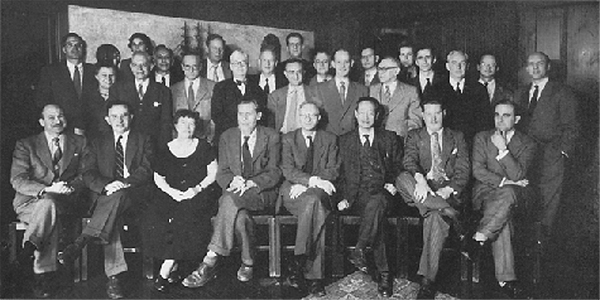
\includegraphics[scale=0.2]{../foto.jpg}
    \end{figure}
    
    
    % ====== DATE ================
    {\large Abril 2018}\\[2cm] 

    \vfill

\end{titlepage}

% =====================================================
% ==========      RESTORE TO DOCUMENT      ============
% =====================================================
\restoregeometry                                                    %Restores the geometry
\nopagecolor                                                        %Use to restore the color to white




% =====================================================
% ========                INDICE              =========
% =====================================================
\tableofcontents{}
\label{sec:Index}

\clearpage

	
	\section{Introducción}
    	Uno de los típicos problemas dentro de un curso de programación es el ordenamiento. Estos algoritmos son la base de muchos otros, además de que tenemos con ellos unas ideas interesantes a usar en otro tipo de algoritmos, como divide y vencerás, las estructuras de datos y los algoritmos aleatorios.
    	
    	
    	Tenemos que tener en cuenta que las computadoras pasan más tiempo ordenando que haciendo otra cosa, sigue siendo el problema de algoritmo combinatorio, también llamado de optimización combinatoria, más presente en el mundo. Como resultado de su estudio existen varias maneras de realizarlo, cada una con una ventaja sobre las demás.
    	
    	\subsection{Métodos}
    	Veamos unos cuantos con un ejemplo de un arco iris.
    	
    	Como debemos saber el arco iris se ordena por su frecuencia:
    	\begin{figure}[h]
                        \centering
                        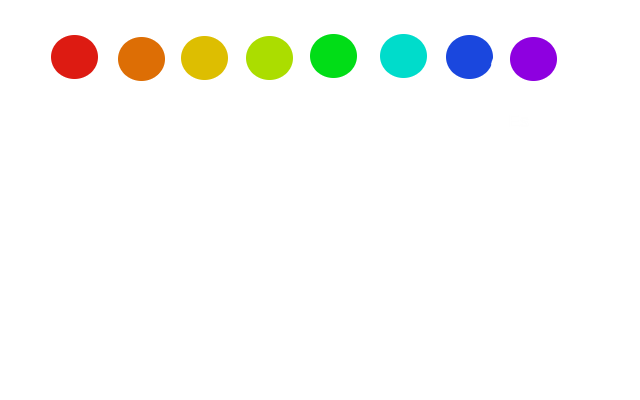
\includegraphics[width=0.4\textwidth]{graphics/Ordenados.png}
                    \end{figure}
                    
                    
        Empecemos con un arco iris desordenado que siempre será el mismo para cada método.
        
            	\begin{figure}[h]
                        \centering
                        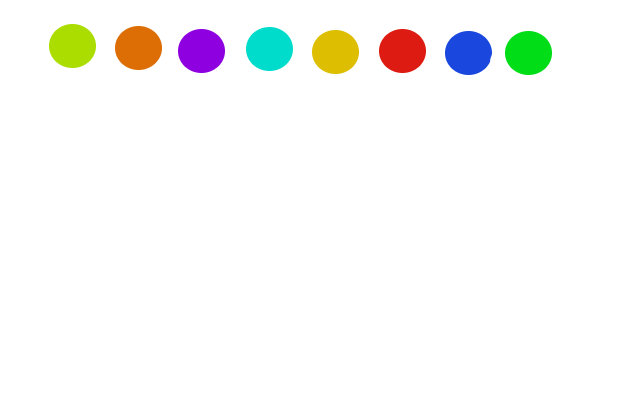
\includegraphics[width=0.4\textwidth]{graphics/Desorden2.png}
                    \end{figure}
    	
    	\subsubsection{Bubble Sort}
    	Este es hacer simplemente un intercambio comparando de dos en dos
    	    
    	    	\begin{figure}[h]
                        \centering
                        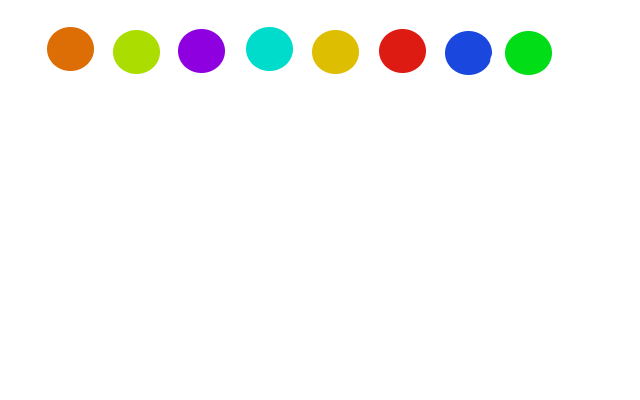
\includegraphics[width=0.4\textwidth]{graphics/Burbuja1-1.png}
                    \end{figure}
                \begin{figure}[h]
                        \centering
                        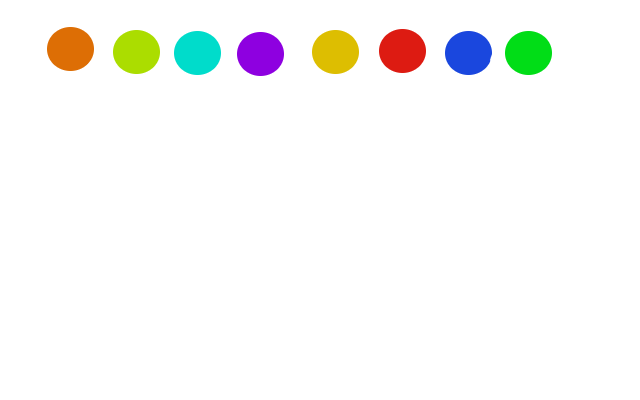
\includegraphics[width=0.4\textwidth]{graphics/Burbuja1-3.png}
                    \end{figure}
                     \clearpage
        \subsubsection{Bubble Sort v2}
        Lo mismo que el anterior solo que asumimos que despues de la primera vuelta el ultimo ya esta ordenado asi que no necesitamos compararlo.
        \begin{figure}[h]
                        \centering
                        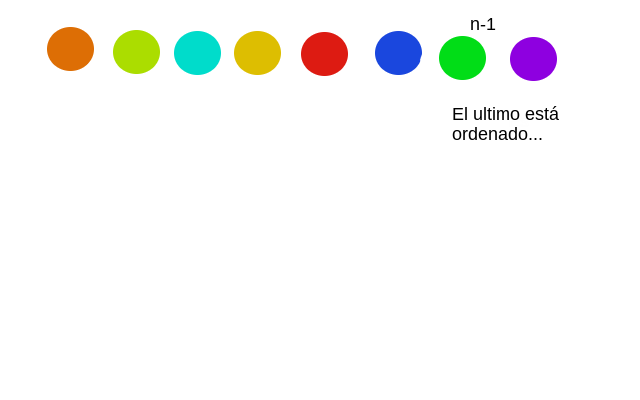
\includegraphics[width=0.4\textwidth]{graphics/Burbuja2-3.png}
                    \end{figure}
                    
        \subsubsection{Bubble Sort v3}
        Simplemente checamos que no este ordenado ya.
        
        \begin{figure}[h]
                        \centering
                        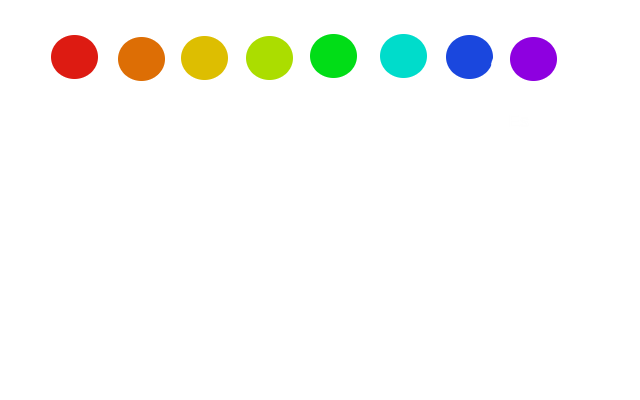
\includegraphics[width=0.4\textwidth]{graphics/Ordenados.png}
                    \end{figure}
        \subsubsection{Selection Sort}
        Selecciona el más pequeño y lo coloca hasta el principio.
        \begin{figure}[h]
                        \centering
                        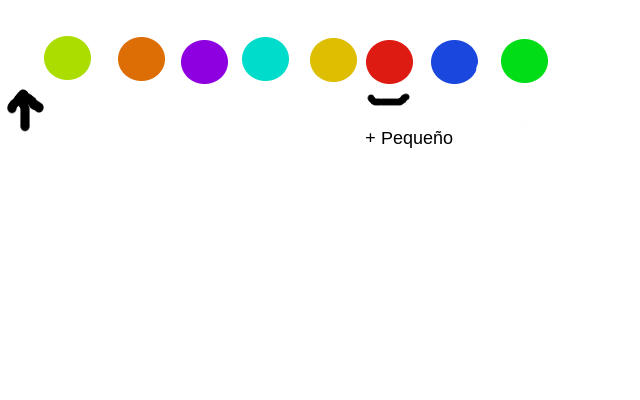
\includegraphics[width=0.4\textwidth]{graphics/Selection-1.png}
                    \end{figure}
        \begin{figure}[h]
                        \centering
                        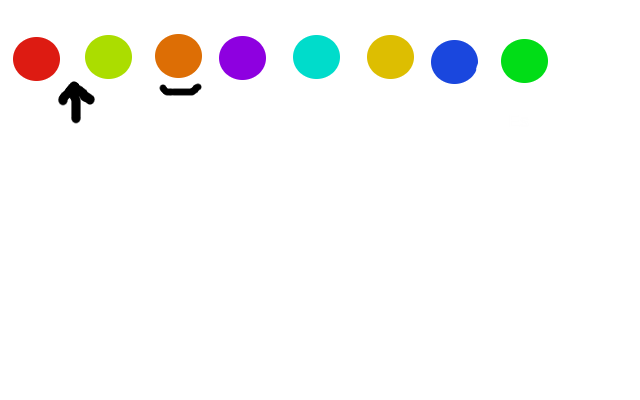
\includegraphics[width=0.4\textwidth]{graphics/Selection-2.png}
                    \end{figure}
    	\begin{figure}[h]
                        \centering
                        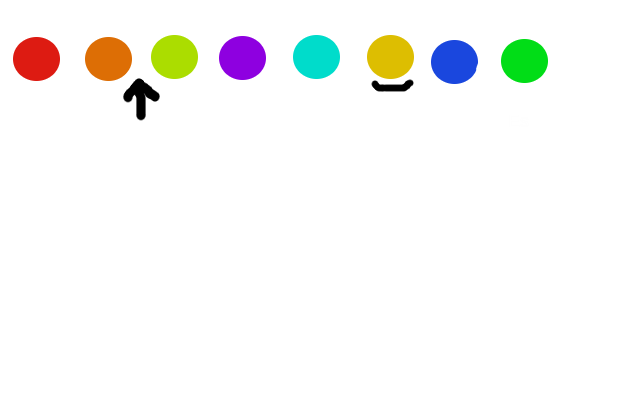
\includegraphics[width=0.4\textwidth]{graphics/Selection-3.png}
                    \end{figure}

 \clearpage
                    
        \subsubsection{Insertion Sort}
        Este es parecido al selection, solo que esta vez buscamos el lugar correcto para cada color en vez de buscar el más pequeño.
        \begin{figure}[h]
                        \centering
                        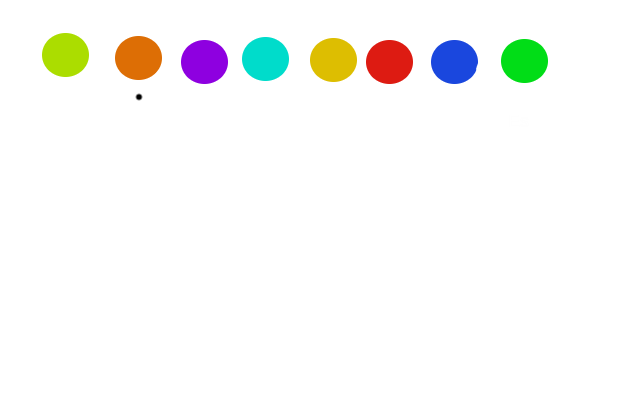
\includegraphics[width=0.4\textwidth]{graphics/Insertion-1.png}
                    \end{figure}
    
    	\begin{figure}[h]
                        \centering
                        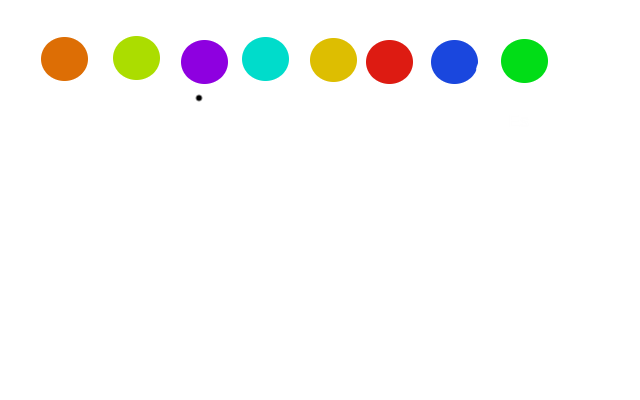
\includegraphics[width=0.4\textwidth]{graphics/Insertion-2.png}
                    \end{figure}
    
    	\begin{figure}[h]
                        \centering
                        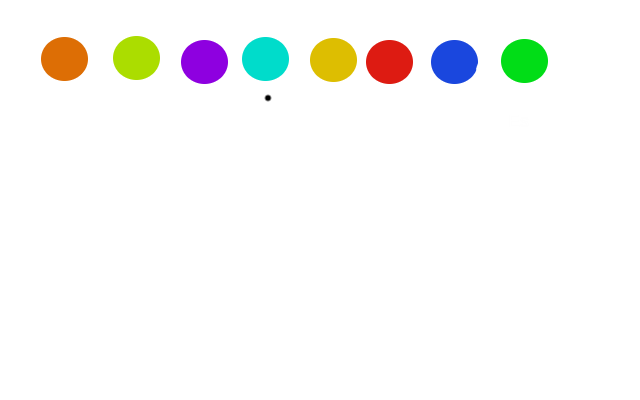
\includegraphics[width=0.4\textwidth]{graphics/Insertion-3.png}
                    \end{figure}
    
    	\begin{figure}[h]
                        \centering
                        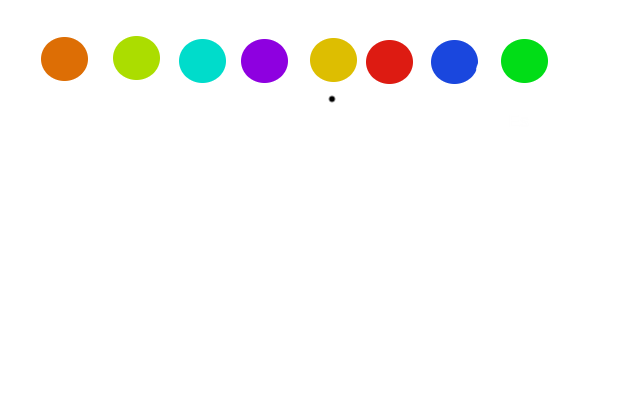
\includegraphics[width=0.4\textwidth]{graphics/Insertion-4.png}
                    \end{figure}
    
    	\begin{figure}[h]
                        \centering
                        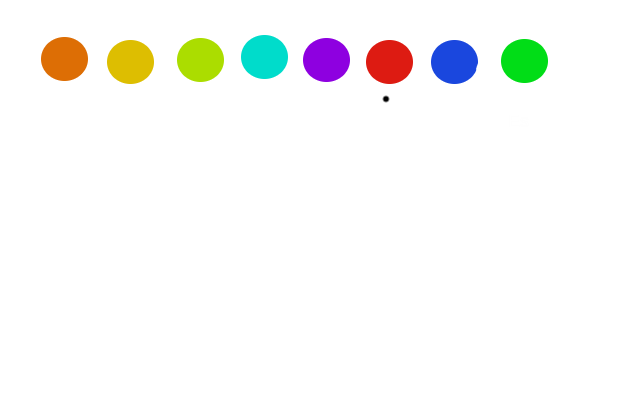
\includegraphics[width=0.4\textwidth]{graphics/Insertion-5.png}
                    \end{figure}
                     \clearpage
                    
        \subsubsection{Shell Sort}
        Un poco mas complejo de entender pero,tomamos saltos compararemos por ejemplo el 1 y 4 y los ordenaremos, despues el 4 y el 8 y asi sucesivamente hasta que todos esten ordenados, bajamos el salto a 3 y asi sucesivamente.
        \begin{figure}[h]
                        \centering
                        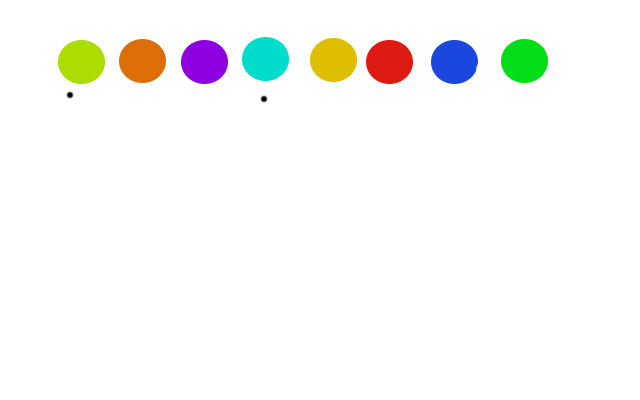
\includegraphics[width=0.4\textwidth]{graphics/Shell1.png}
                    \end{figure}
    	
    	\begin{figure}[h]
                        \centering
                        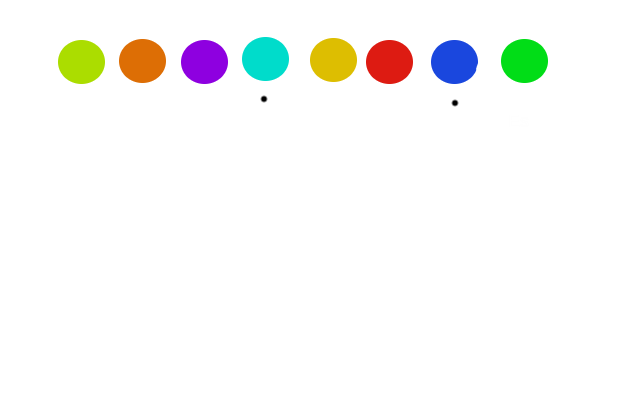
\includegraphics[width=0.4\textwidth]{graphics/Shell2.png}
                    \end{figure}
    
    	\begin{figure}[h]
                        \centering
                        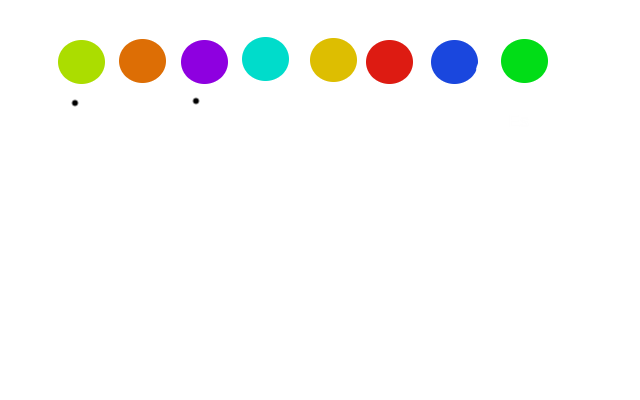
\includegraphics[width=0.4\textwidth]{graphics/Shell3.png}
                    \end{figure}
    	
    	\begin{figure}[h]
                        \centering
                        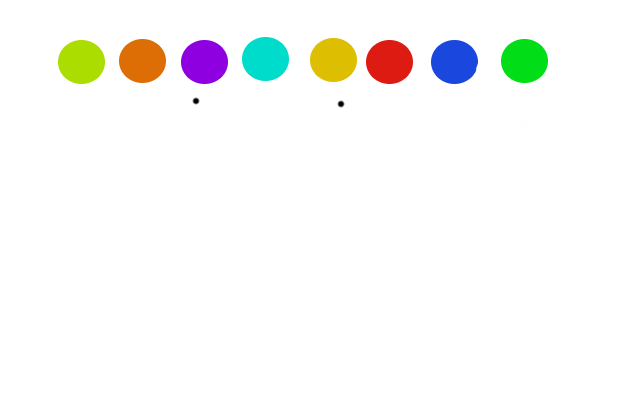
\includegraphics[width=0.4\textwidth]{graphics/Shell4.png}
                    \end{figure}
    	
    	\begin{figure}[h]
                        \centering
                        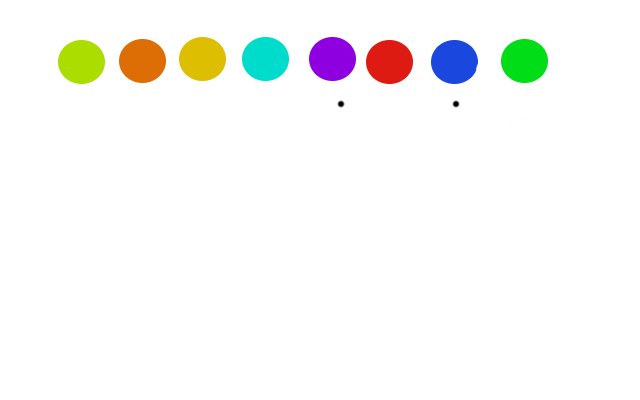
\includegraphics[width=0.4\textwidth]{graphics/Shell5.png}
                    \end{figure}
                     \clearpage
    	\subsubsection{BTS}
    	Metemos el arreglo en un arbol y lo recorremos en inorden.
    	\begin{figure}[h]
                        \centering
                        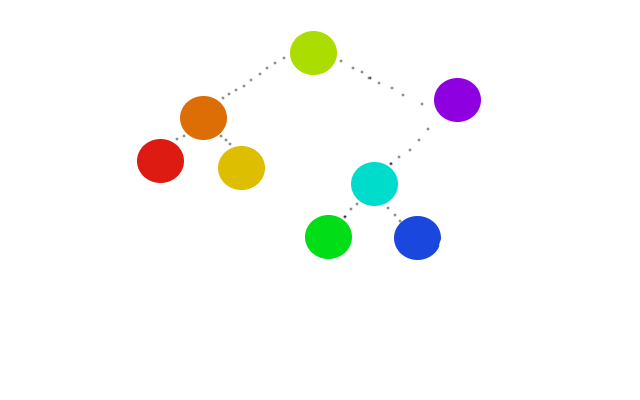
\includegraphics[width=0.4\textwidth]{graphics/Arbol-1.png}
                    \end{figure}
    	\begin{figure}[h]
                        \centering
                        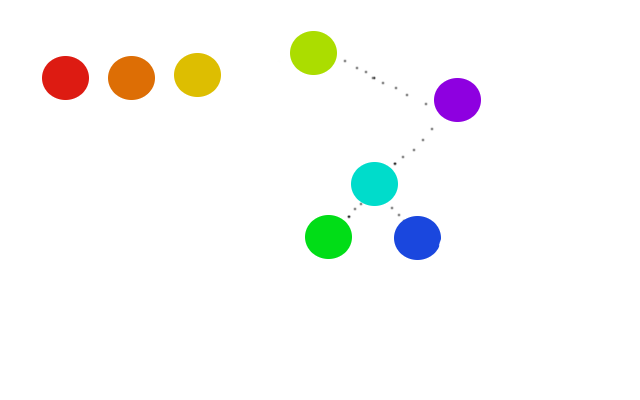
\includegraphics[width=0.4\textwidth]{graphics/Arbol-2.png}
                    \end{figure}
                     \clearpage
    	
        
    	\subsection{Definición}
    	
    	
    	    Dado un arreglo $A[0, 1, \ldots, n-1]$ de longitud $n \in \mathbb{N}$ de cualquier tipo de elementos sobre los cuales es posible aplicar una relación de orden total $\leq$, decimos que está \textbf{ordenado} si \cite{ref1}:
    	    \begin{align*}
    	        i < j \quad \implies \quad A[i] \leq A[j]
    	    \end{align*}
    	    
    	    Es decir, si $A$ está ordenado podemos decir que $A[0] \leq A[1] \leq \cdots \leq A[n-1]$. Por convención, consideraremos a los arreglos de tamaño 0 y 1 como ordenados trivialmente.
    	    
    	    En esta práctica consideraremos a los elementos de $A$ como números enteros.
    	
    	\subsection{Algoritmo de ordenamiento}
    	    Es un algoritmo que recibe un arreglo $A[0, 1, \ldots, n-1]$ y devuelve una permutación ordenada de $A$, llamémosle $B$, tal que $B[0] \leq B[1] \leq \cdots \leq B[n-1]$. En la práctica el arreglo $B$ se sobreescribe a $A$. Más formalmente, este algoritmo calcula de forma indirecta una función de \emph{permutación ordenadora} de los índices de $A$, $\sigma : \{0, 1, \ldots, n-1\} \to \{0, 1, \ldots, n-1\}$, tal que $A[\sigma(0)] \leq A[\sigma(1)] \leq \cdots \leq A[\sigma(n-1)]$.
    	    
    	    Decimos que un algoritmo de ordenamiento es \textbf{estable} si:
    	    \begin{align*}
    	        i < j \text{ y } A[i] = A[j] \quad \implies \quad \sigma(i) \leq \sigma(j)
    	    \end{align*}
    	    Es decir, los elementos iguales mantienen sus posiciones relativas despúes de ordenar el arreglo.
    	    
    	\subsection{Algoritmos famosos}
    	    
    	    
	
	
	\section{Planteamiento del problema}
	    
	    Con base en el archivo de entrada proporcionado que tiene \textbf{10,000,000 de números diferentes}, ordenarlo bajo los siguientes métodos de ordenamiento y comparar experimentalmente las complejidades de estos:
	    \begin{itemize}\setlength\itemsep{0em}
	        \item Burbuja (Bubble Sort) \begin{itemize}\setlength\itemsep{0em}
	            \item Burbuja Simple
	            \item Burbuja Optimizada
	        \end{itemize}
	        \item Inserción (Insertion Sort)
	        \item Selección (Selection Sort)
	        \item Shell (Shell Sort)
	        \item Ordenamiento con árbol binario de búsqueda (Tree Sort)
	    \end{itemize}

	

    \clearpage

	\section{Diseño de la solución}
		\subsection{Burbuja}
        	\begin{algorithm}[H]
            \caption{Burbuja Simple}
            \begin{algorithmic}[1]
                \Procedure{BubbleSortV1}{$A,n$}
                \For{$i \gets 0$ hasta $n-2$}
                    \For{$j \gets 0$ hasta $n-2$}
                        \If{$A[j] > A[j+1]$}
                            \State $aux \gets A[j]$
                            \State $A[j] \gets A[j+1]$
                            \State $A[j+1] \gets aux$
                        \EndIf
                    \EndFor
                \EndFor
                \EndProcedure
                \end{algorithmic}
            \end{algorithm}
            
            \begin{algorithm}[H]
            \caption{Burbuja Optimizada}
            \begin{algorithmic}[1]
                \Procedure{BubbleSortV2}{$A,n$}
                \For{$i \gets 0$ hasta $n-2$}
                    \For{$j \gets 0$ hasta $n-i-2$}
                        \If{$A[j] > A[j+1]$}
                            \State $aux \gets A[j]$
                            \State $A[j] \gets A[j+1]$
                            \State $A[j+1] \gets aux$
                        \EndIf
                    \EndFor
                \EndFor
                \EndProcedure
                \end{algorithmic}
            \end{algorithm}
            
            \begin{algorithm}[H]
            \caption{Burbuja Optimizada}
            \begin{algorithmic}[1]
                \Procedure{BubbleSortV3}{$A,n$}
                \For{$i \gets 0$ hasta $n-2$}
                    \State cambio $\gets$ NO
                    \For{$j \gets 0$ hasta $n-i-2$}
                        \If{$A[j] > A[j+1]$}
                            \State $aux \gets A[j]$
                            \State $A[j] \gets A[j+1]$
                            \State $A[j+1] \gets aux$
                            \State $cambio \gets$ SÍ
                        \EndIf
                    \EndFor
                    \If{$cambio$ = NO}
                        \State \textbf{Salir}
                    \EndIf
                \EndFor
                \EndProcedure
                \end{algorithmic}
            \end{algorithm}
            
		\subsection{Inserción}
            \begin{algorithm}[H]
            \caption{Inserción}
            \begin{algorithmic}[1]
                \Procedure{InsertionSort}{$A,n$}
                \For{$i \gets 1$ hasta $n-1$}
                    \State $j \gets i$
                    \State $Temp \gets A[i]$
                    \While{$j > 0$ y $Temp < A[j - 1]$}
                        \State $A[j] \gets A[j - 1]$
                        \State $j \gets j - 1$
                    \EndWhile
                    \State $A[j] \gets Temp$
                \EndFor
                \EndProcedure
                \end{algorithmic}
            \end{algorithm}
            
		\subsection{Selección}
            \begin{algorithm}[H]
            \caption{Selección}
            \begin{algorithmic}[1]
                \Procedure{SelectionSort}{$A,n$}
                \For{$i \gets 0$ hasta $n-2$}
                    \State $Smallest \gets i$
                    \For{$j \gets i + 1$ hasta $n-1$}
                        \If{$A[j] < A[Smallest]$}
                            \State $Smallest \gets j$
                        \EndIf
                    \EndFor
                    \State $aux \gets A[Smallest]$
                    \State $A[Smallest] \gets A[i]$
                    \State $A[i] \gets aux$
                \EndFor
                \EndProcedure
                \end{algorithmic}
            \end{algorithm}
            
		\subsection{Shell}
            \begin{algorithm}[H]
            \caption{Shell}
            \begin{algorithmic}[1]
                \Procedure{ShellSort}{$A,n$}
                \State $Gap \gets \lfloor \frac{n}{2} \rfloor$
                \While{$Gap > 0$}
                    \For{$i \gets Gap$ hasta $n-1$}
                        \State $j \gets i$
                        \State $Temp \gets A[i]$
                        \While{$j \geq Gap$ y $Temp < A[j - Gap]$}
                            \State $A[j] \gets A[j - Gap]$
                            \State $j \gets j - Gap$
                        \EndWhile
                        \State $A[j] \gets Temp$
                    \EndFor
                    \State $Gap \gets \lfloor \frac{Gap}{2} \rfloor$
                \EndWhile
                \EndProcedure
                \end{algorithmic}
            \end{algorithm}
            
		\subsection{Árbol binario de búsqueda}
            \begin{algorithm}[H]
            \caption{Árbol binario de búsqueda}
            \begin{algorithmic}[1]
                \Procedure{InsertBST}{$Arbol, elemento$}
                    \State $posicion \gets Arbol$
                    \While{$posicion \neq NULL$}
                        \If{$elemento < posicion.elemento$}
                            \State $posicion \gets posicion.izquierda$
                        \Else
                            \State $posicion \gets posicion.derecha$
                        \EndIf
                    \EndWhile
                    \State $posicion \gets \textbf{NuevoNodo}(elemento)$
                \EndProcedure
                \Procedure{Inorder}{$Arbol, A, n$}
                    \State $posicion \gets Arbol$
                    \State $i \gets 0$
                    \State $pila \gets \{\}$
                    \Do
                        \While{$posicion \neq NULL$}
                            \State $pila.push(posicion)$
                            \State $posicion \gets posicion.izquierda$
                        \EndWhile
                        \If{$pila$ es no vacía}
                            \State $posicion \gets pila.pop()$
                            \State $A[i] \gets posicion.elemento$
                            \State $i \gets i + 1$
                            \State $posicion \gets posicion.derecha$
                        \EndIf
                    \doWhile{$posicion \neq NULL$ y $pila$ es no vacía}
                \EndProcedure
                \Procedure{SortWithBST}{$A, n$}
                    \State $Arbol \gets NULL$
                    \For{$i \gets 0$ hasta $n-1$}
                        \State $\textbf{InsertBST}(Arbol, A[i])$
                    \EndFor
                    \State $\textbf{Inorder}(Arbol, A, n)$
                \EndProcedure
                \end{algorithmic}
            \end{algorithm}
	
    \clearpage
    
	\section{Implementación de la solución}
	
	    \subsection{Burbuja}
	        \inputminted[breaklines, linenos, tabsize=4, fontsize=\footnotesize, firstline=29, lastline=36, firstnumber=1]{c}{code/BubbleSort.c}
	        
	        \inputminted[breaklines, linenos, tabsize=4, fontsize=\footnotesize, firstline=49, lastline=56, firstnumber=1]{c}{code/BubbleSort.c}
	        
	        \inputminted[breaklines, linenos, tabsize=4, fontsize=\footnotesize, firstline=68, lastline=82, firstnumber=1]{c}{code/BubbleSort.c}
	    
	    \subsection{Inserción}
	        \inputminted[breaklines, linenos, tabsize=4, fontsize=\footnotesize, firstline=30, lastline=44, firstnumber=1]{c}{code/InsertionSort.c}
	        
	    \subsection{Selección}
	        \inputminted[breaklines, linenos, tabsize=4, fontsize=\footnotesize, firstline=29, lastline=39, firstnumber=1]{c}{code/SelectionSort.c}
	        
	    \subsection{Shell}
	        \inputminted[breaklines, linenos, tabsize=4, fontsize=\footnotesize, firstline=33, lastline=53, firstnumber=1]{c}{code/ShellSort.c}
	        
	    \subsection{Árbol binario de búsqueda}
	        \inputminted[breaklines, linenos, tabsize=4, fontsize=\footnotesize, firstline=16, lastline=22, firstnumber=1]{c}{code/TreeAuxFunction.c}
	        
	        \inputminted[breaklines, linenos, tabsize=4, fontsize=\footnotesize, firstline=37, lastline=43, firstnumber=1]{c}{code/TreeAuxFunction.c}
	        
	        \inputminted[breaklines, linenos, tabsize=4, fontsize=\footnotesize, firstline=58, lastline=66, firstnumber=1]{c}{code/TreeAuxFunction.c}
	        
	        \inputminted[breaklines, linenos, tabsize=4, fontsize=\footnotesize, firstline=80, lastline=103, firstnumber=1]{c}{code/TreeAuxFunction.c}
	        
	        \inputminted[breaklines, linenos, tabsize=4, fontsize=\footnotesize, firstline=26, lastline=33, firstnumber=1]{c}{code/SortWithBST.c}
	
	\clearpage
	
	\section{Actividades y pruebas}
	
	    \subsection{Comparativas individuales}
	    
    	    \subsubsection{Burbuja}
    	        \begin{figure}[H]
    	            \centering
    	            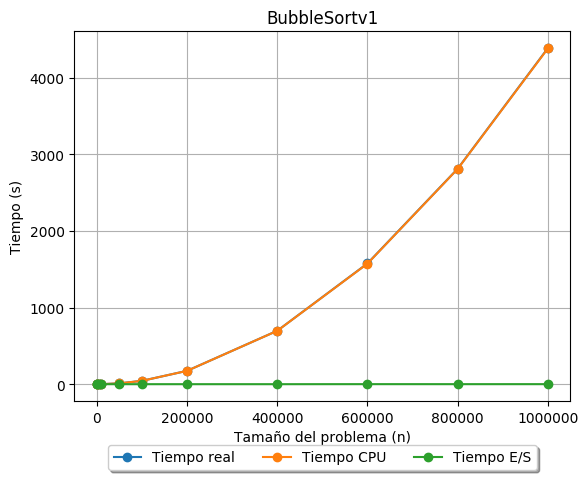
\includegraphics[scale=0.78]{graphics/BubbleSortv1-ExperimentalTimes.png}
    	        \end{figure}
    	        
    	        \begin{figure}[H]
    	            \centering
    	            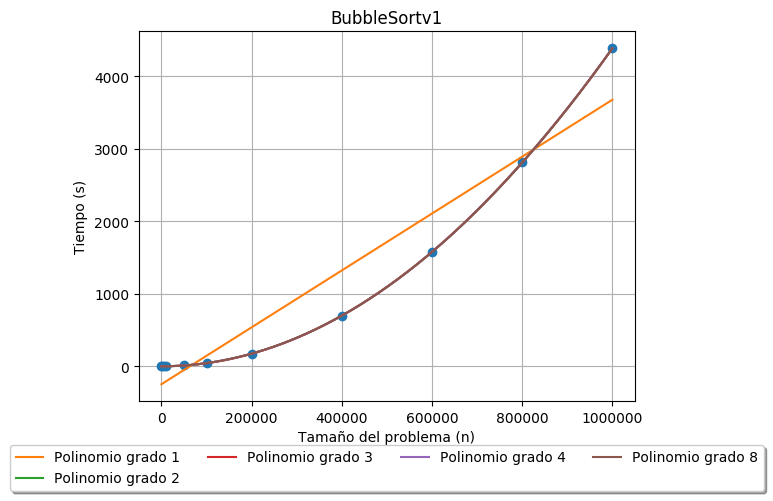
\includegraphics[scale=0.78]{graphics/BubbleSortv1-Polynomials.png}
    	        \end{figure}
    	        
    	        \begin{figure}[H]
    	            \centering
    	            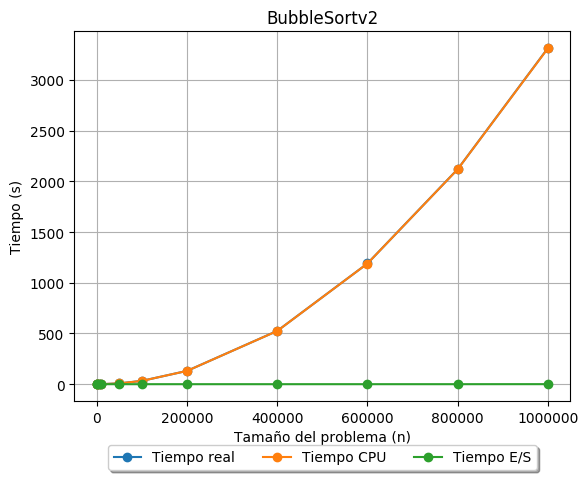
\includegraphics[scale=0.9]{graphics/BubbleSortv2-ExperimentalTimes.png}
    	        \end{figure}
    	        
    	        \begin{figure}[H]
    	            \centering
    	            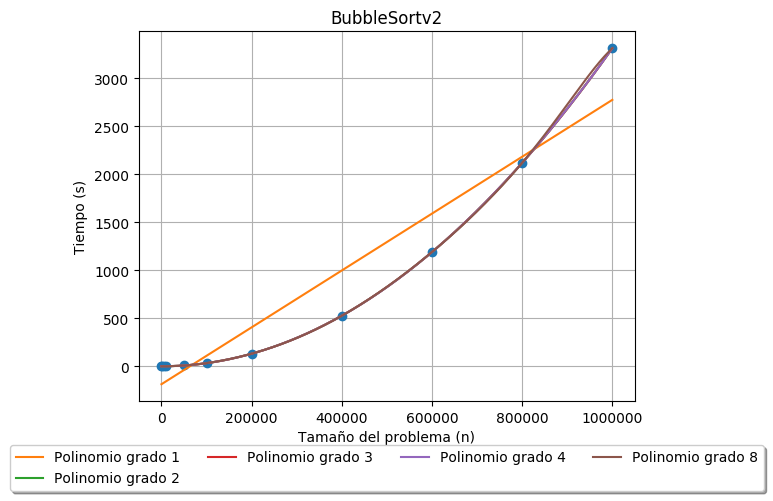
\includegraphics[scale=0.9]{graphics/BubbleSortv2-Polynomials.png}
    	        \end{figure}
    	        
    	        \begin{figure}[H]
    	            \centering
    	            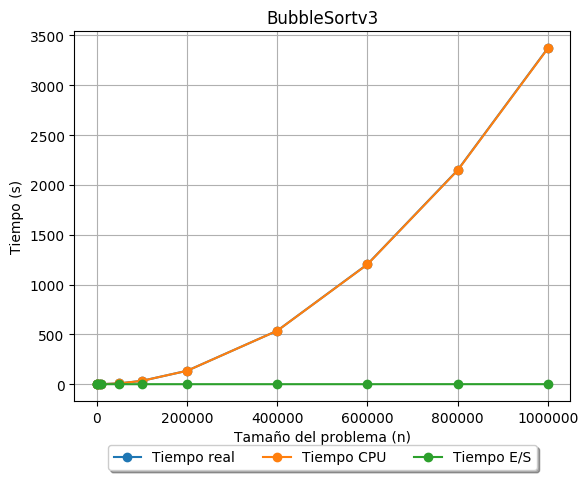
\includegraphics[scale=0.9]{graphics/BubbleSortv3-ExperimentalTimes.png}
    	        \end{figure}
    	        
    	        \begin{figure}[H]
    	            \centering
    	            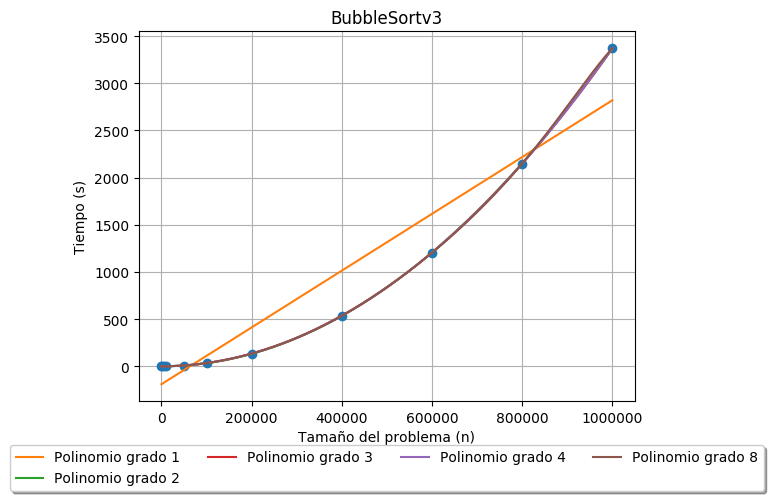
\includegraphics[scale=0.9]{graphics/BubbleSortv3-Polynomials.png}
    	        \end{figure}
    	        
    	   \subsubsection{Inserción}
    	        \begin{figure}[H]
    	            \centering
    	            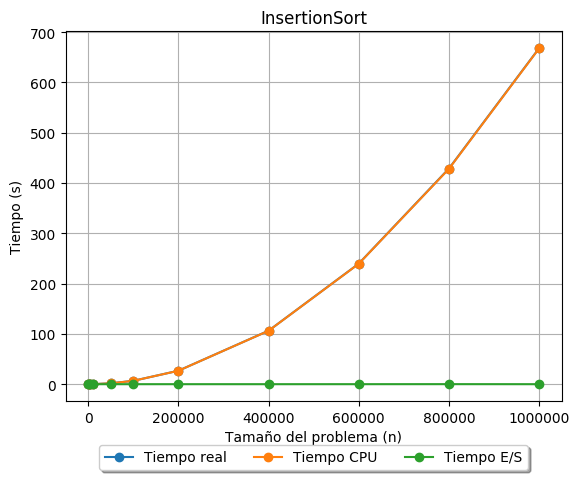
\includegraphics[scale=0.86]{graphics/InsertionSort-ExperimentalTimes.png}
    	        \end{figure}
    	        
    	        \begin{figure}[H]
    	            \centering
    	            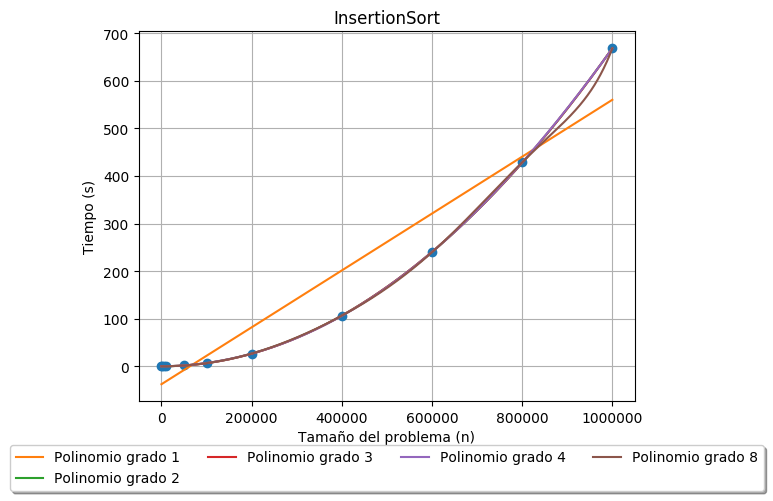
\includegraphics[scale=0.86]{graphics/InsertionSort-Polynomials.png}
    	        \end{figure}
    	        
    	   \subsubsection{Selección}
    	        \begin{figure}[H]
    	            \centering
    	            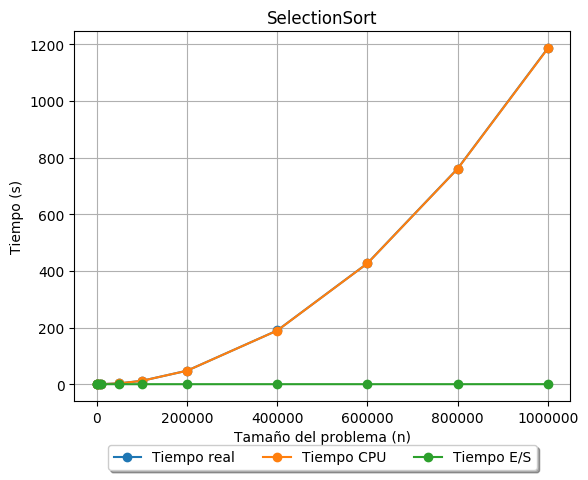
\includegraphics[scale=0.86]{graphics/SelectionSort-ExperimentalTimes.png}
    	        \end{figure}
    	        
    	        \begin{figure}[H]
    	            \centering
    	            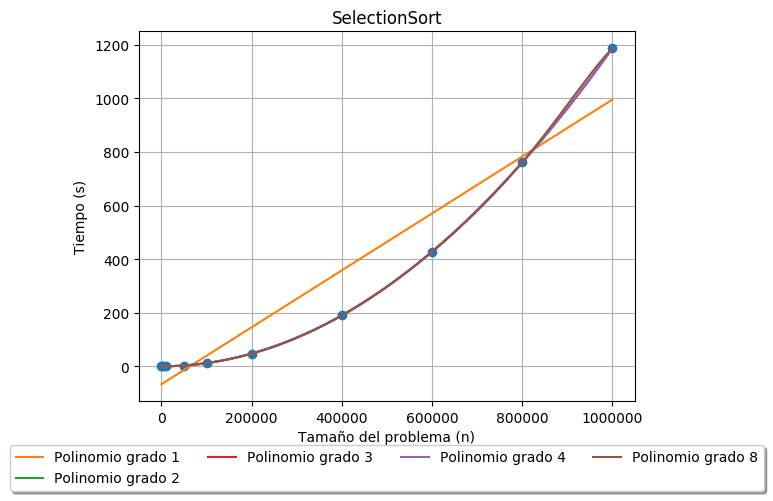
\includegraphics[scale=0.86]{graphics/SelectionSort-Polynomials.png}
    	        \end{figure}
    	        
    	    \subsubsection{Shell}
    	        \begin{figure}[H]
    	            \centering
    	            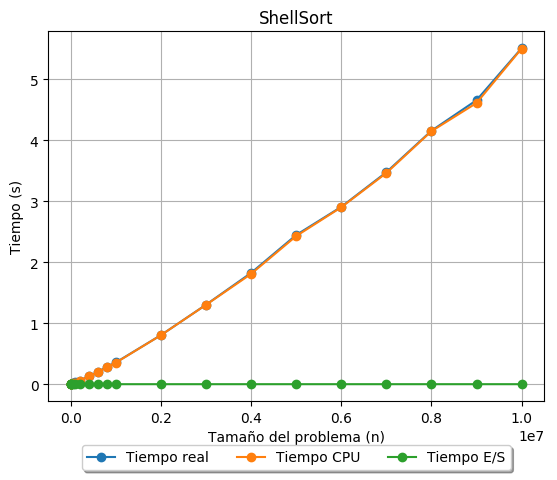
\includegraphics[scale=0.86]{graphics/ShellSort-ExperimentalTimes.png}
    	        \end{figure}
    	        
    	        \begin{figure}[H]
    	            \centering
    	            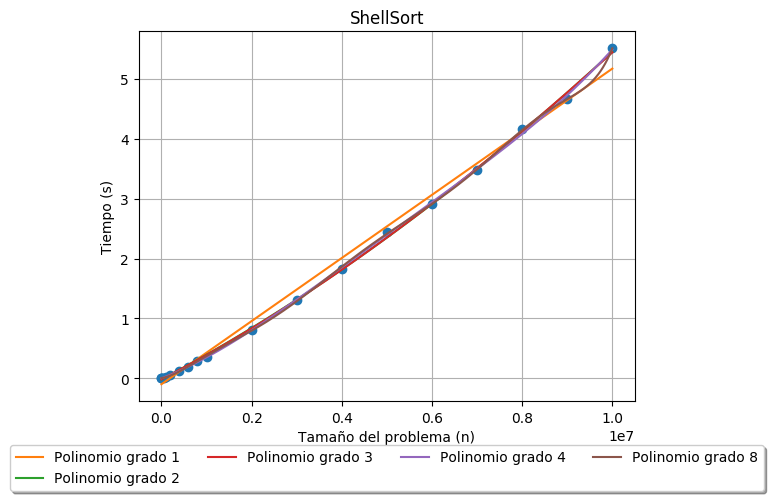
\includegraphics[scale=0.86]{graphics/ShellSort-Polynomials.png}
    	        \end{figure}
    	        
    	    \subsubsection{Árbol binario de búsqueda}
    	        \begin{figure}[H]
    	            \centering
    	            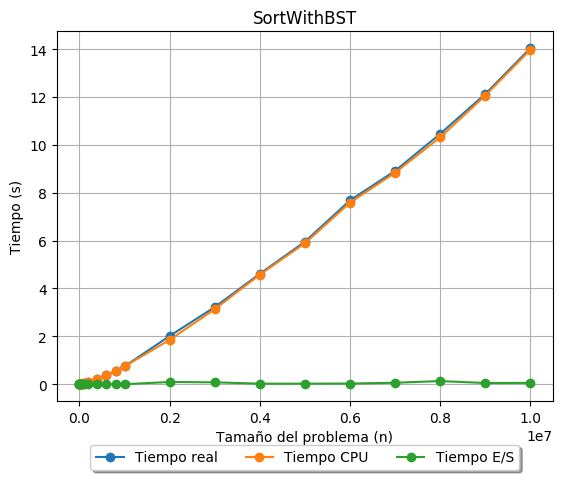
\includegraphics[scale=0.86]{graphics/SortWithBST-ExperimentalTimes.png}
    	        \end{figure}
    	        
    	        \begin{figure}[H]
    	            \centering
    	            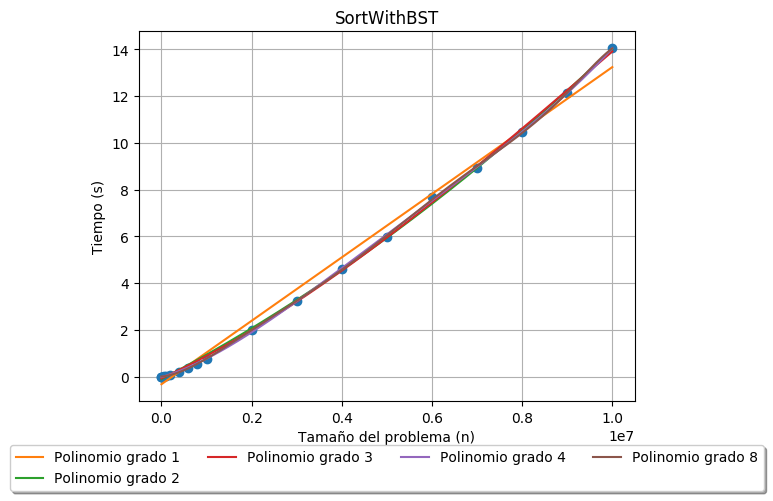
\includegraphics[scale=0.86]{graphics/SortWithBST-Polynomials.png}
    	        \end{figure}
    	        
    	        
	    \subsection{Comparativas globales}
	    
	        \subsubsection{Por tiempo real}
	            \begin{figure}[H]
    	            \centering
    	            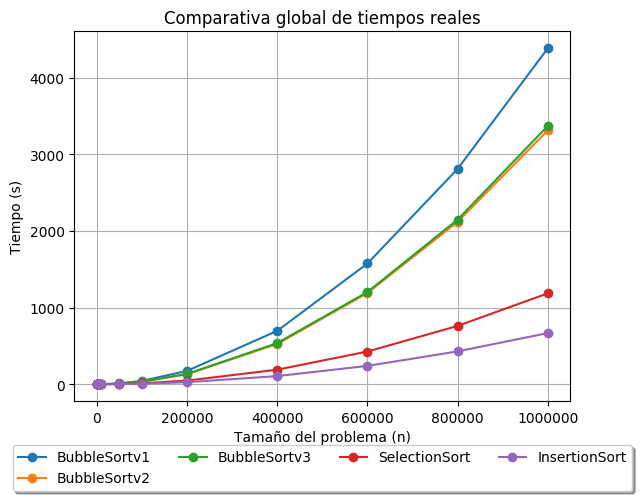
\includegraphics[scale=0.78]{graphics/globalComparativeTimes2.png}
    	        \end{figure}
    	        
    	        \begin{figure}[H]
    	            \centering
    	            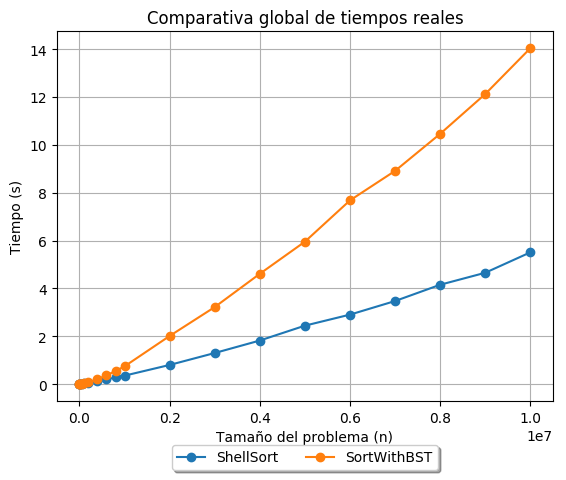
\includegraphics[scale=0.78]{graphics/globalComparativeTimes3.png}
    	        \end{figure}
    	        
    	        \begin{figure}[H]
    	            \centering
    	            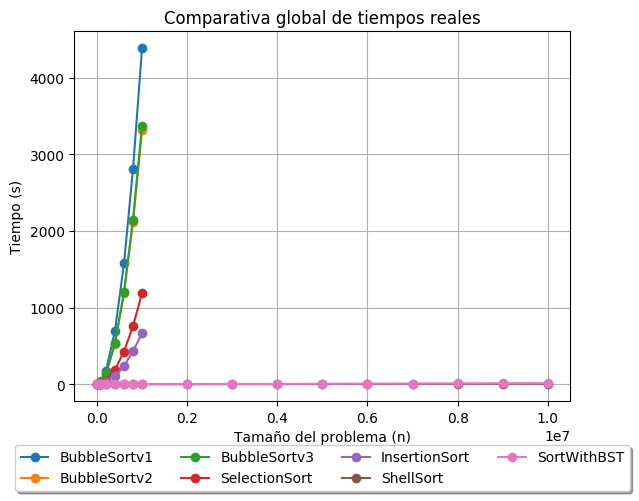
\includegraphics[scale=0.9]{graphics/globalComparativeTimes1.png}
    	        \end{figure}
    	        
    	  \clearpage
	        
	        \subsubsection{Por polinomio}
	            \begin{figure}[H]
    	            \centering
    	            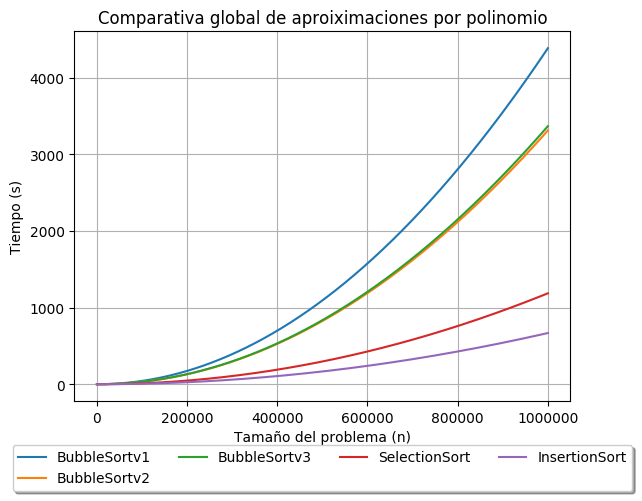
\includegraphics[scale=0.84]{graphics/globalComparativePolynomial2.png}
    	        \end{figure}
    	        
    	        \begin{figure}[H]
    	            \centering
    	            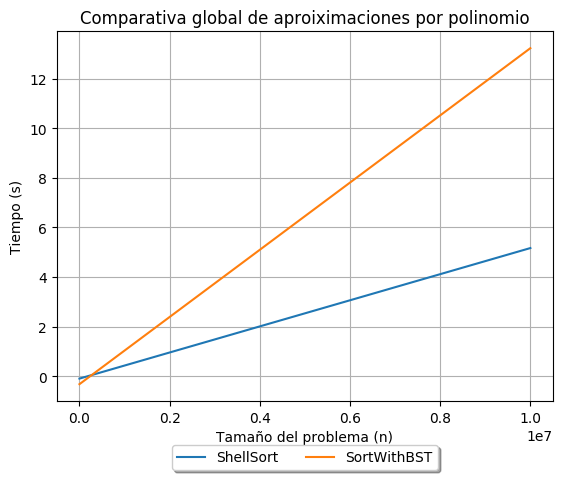
\includegraphics[scale=0.84]{graphics/globalComparativePolynomial3.png}
    	        \end{figure}
    	        
    	        \begin{figure}[H]
    	            \centering
    	            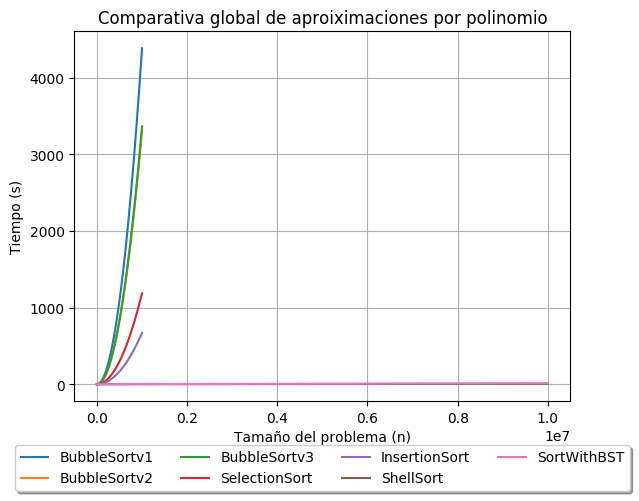
\includegraphics[scale=0.9]{graphics/globalComparativePolynomial1.png}
    	        \end{figure}
    	        
    	        
    	    Los polinomios escogidos como mejores aproximaciones fueron:
    	    \begin{itemize}\setlength\itemsep{0em}
    	        \item BubbleSort v1:
    	        
    	        $P(n) = 4.39614394 \times 10^{-9} n^2 - 9.38843814 \times 10^{-6} n + 0.06536545$
    	        
    	        \item BubbleSort v2:
    	        
    	        $P(n) = 3.32645251 \times 10^{-9} n^2 - 1.30521594 \times 10^{-5} n + 0.19869421$
    	        
    	        \item BubbleSort v3:
    	        
    	        $P(n) = 3.39403986 \times 10^{-9} n^2 - 2.61286379 \times 10^{-5} n + 1.00078946$
    	        
    	        \item SelectionSort:
    	        
    	        $P(n) = 1.18611115 \times 10^{-9} n^2 + 1.05506770 \times 10^{-6} n - 0.02919735$
    	        
    	        \item InsertionSort:
    	        
    	        $P(n) = 6.70213950 \times 10^{-10} n^2 - 1.77898112 \times 10^{-6} n + 0.04638817$
    	        
    	        \item ShellSort:
    	        
    	        $P(n) = 5.26723624 \times 10^{-7} n - 0.09826119$
    	        
    	        \item SortWithBST:
    	        
    	        $P(n) = 1.35578423 \times 10^{-6} n - 0.32358203$
    	    \end{itemize}
    	    
    	    Para los primeros 5 algoritmos escogimos un polinomio cuadrático, pues es lo más cercano a la complejidad del caso medio, $O(n^2)$.
    	    
    	    Para los últimos dos usamos un polinomio lineal, pues es el más cercano a la complejidad teórica de $O(n \log n)$ en el caso medio.
    	    
    	    Si usamos esos polinomios para estimar los tiempos para valores de $n$ mucho más grandes, obtenemos los siguientes tiempos estimados:
    	    
    	    \begin{table}[H]
    	        \centering
    	        \begin{tabular}{|c|c|c|c|c|c|}
    	             \hline
    	             & $n = 5 \times 10^{-7}$ & $n = 10^{8}$ & $n = 5 \times 10^{8}$ & $n = 10^{9}$ & $n = 5 \times 10^{9}$ \\ \hline
    	             BubbleSortv1 & 10,989,890.5 s & 43,960,500.6 s & 1,099,031,292.4 s & 4,396,134,557.8 s & 109,903,551,713.3 s \\ \hline
    	             BubbleSortv2 & 8,315,478.8 s & 33,263,220.1 s & 831,606,602.4 s & 3,326,439,461.2 s & 83,161,247,570.3 s \\ \hline
    	             BubbleSortv3 & 8,483,794.2 s & 33,937,786.7 s & 848,496,902.9 s & 3,394,013,737.5 s & 84,850,865,987.1 s \\ \hline
    	             SelectionSort & 2,965,330.6 s & 11,861,217.0 s & 296,528,315.7 s & 1,186,112,208.2 s & 29,652,784,104.6 s \\ \hline
    	             InsertionSort & 1,675,445.9 s & 6,701,961.6 s & 167,552,598.0 s & 670,212,171.0 s & 16,755,339,855.5 s \\ \hline
    	             ShellSort & 26.2 s & 52.5 s & 263.2 s & 526.6 s & 2,633.5 s \\ \hline
    	             SortWithBST & 67.4 s & 135.2 s & 677.5 s & 1,355.4 s & 6,778.5 s \\ \hline
    	        \end{tabular}
    	    \end{table}
    	        

        \clearpage
        
	    \subsection{Preguntas}
	    
	        \begin{enumerate}\setlength\itemsep{0em}
	            \item \textbf{¿Cuál de los 5 algoritmos es más fácil de implementar?}
	            
	                El algoritmo de burbuja en sus tres versiones, porque solo requerimos de realizar intercambios entre elementos consecutivos del arreglo, lo cual es relativamente sencillo.
	            
	            \item \textbf{¿Cuál de los 5 algoritmos es el más difícil de implementar?}
	            
	                El algoritmo con el árbol binario de búsqueda, porque tuvimos que trabajar con punteros, crear una estructura para los nodos, y convertir los procedimientos de inserción y recorrido inorden a sus versiones iterativas.
	            
	            \item \textbf{¿Cuál algoritmo tiene menor complejidad temporal?}
	            
	                Teóricamente el árbol binario de búsqueda, pues en este caso como los números están distribuidos uniformemente, el árbol creado estará más o menos balanceado, logrando la inserción de cada elemento en $O(\log n)$ y la inserción de todos en $O(n \log n)$.
	                
	                Sin embargo, el más rápido en la práctica fue Shell Sort, tomando la mitad de tiempo que el árbol binario de búsqueda. Los saltos escogidos sirvieron para reducir el número de inserciones.
	            
	            \item \textbf{¿Cuál algoritmo tiene mayor complejidad temporal?}
	            
	                BubbleSort versión 1, porque siempre realiza $O(n^2)$ intercambios, sin importar cómo estén distribuidos los elementos del arreglo.
	            
	            \item \textbf{¿Cuál algoritmo tiene menor complejidad espacial? ¿Por qué?}
	            
	                InsertionSort y ShellSort, porque el ordenamiento de los elementos se realiza sobre el mismo arreglo, y como aquí no se realizan intercambios sino solo desplazamientos, no necesitamos memoria extra.
	                
	                Aunque BubbleSort y SelectionSort también realizan el ordenamiento sobre el arreglo, requieren un poco más de memoria para intercambiar elementos, pero la diferencia con los anteriores es casi nula.
	            
	            \item \textbf{¿Cuál algoritmo tiene mayor complejidad espacial? ¿Por qué?}
	            
	                El árbol binario de búsqueda, porque necesitamos construir el árbol, cuya cantidad de nodos es la misma que la de los elementos del arreglo, requiriendo el doble de memoria para ordenarlo. Además, como se usó la versión iterativa del recorrido inorden, tuvimos que hacer una pila para simular la recursión, y como esa pila guarda todos los nodos del árbol, en total usamos el triple de memoria.
	            
	            \item \textbf{¿El comportamiento experimental de los algoritmos era el esperado? ¿Por qué?}
	            
	                \begin{itemize}\setlength\itemsep{0em}
	                    \item El de BubbleSort versión 1 fue el más tardado de todos, lo cuál esperábamos.
	                    \item Las otras dos versiones de BubbleSort tardaron casi lo mismo, pero menos que la versión 1; por lo que la optimización de revisar si ya no habíamos hecho intercambios no fue muy efectiva en este caso.
	                    \item El SelectionSort tardó menos, lo cual también esperábamos, aunque también siempre realice $O(n^2)$ operaciones.
	                    \item El InsertionSort no estuvo nada mal, siendo el más rápido hasta este punto, pues no realiza intercambios, solo desplazamientos; y es eficiente si el arreglo está más o menos ordenado.
	                    \item El ShellSort nos sorprendió, pues fue el más rápido de todos. Al parecer los saltos escogidos fueron los adecuados para reducir drásticamente el tiempo de ordenamiento.
	                    \item El ordenamiento con el BST fue el segundo más rápido, lo cuál esperábamos porque, aparte de insertar cada elemento al árbol, hay que recorrerlo y volverlo a copiar al arreglo original. Tardó el doble que ShellSort.
	                \end{itemize}
	            
	            \item \textbf{¿Sus resultados experimentales difieren mucho de los del resto de los equipos? ¿A qué se debe?}
	            
	            
	            Comprobamos con el equipo Git Gud Team Arbol ,especialmente con Manuel, ejecutamos los códigos gracias al Make.py en la máquina estándar que tiene su equipo y comprobamos que las gráficas son prácticamente iguales, sin importar la implementación el compilador llego básicamente al mismo programa ejecutable.
	            
	            Por otro lado si que tenemos diferencias al comprobar los datos cada uno usando sus propios equipos, estas pequeñas diferencias se deben sobretodo a las especificaciones.
	                
	            
	            \item \textbf{¿Existió un entorno controlado para realizar las pruebas experimentales? ¿Cuál fue?}
	            
	                Sí, usamos una PC con las siguientes características:
	                \begin{itemize}\setlength\itemsep{0em}
	                    \item HP EliteDesk 700 G1 SFF
	                    \item 8GB de memoria RAM, DDR3 SDRAM non-ECC, 1600MHz
	                    \item Procesador Intel(R) Core(TM) i5-4590 (4$^\circ$ generación), CPU @ 3.30GHz (4 CPUs), $\sim$3.3GHz. Intel vPro Technology
	                    \item 1TB de disco duro HDD, Serial ATA-600 6Gb/s, 7200 rpm
	                \end{itemize}
	                
	                Y el software fue el siguiente:
	                \begin{itemize}\setlength\itemsep{0em}
	                    \item Sistema operativo Linux
	                    \item Distribución Elementary OS 0.4
	                    \item Compliador GCC con soporte para C11
	                    \item Python 3.6 con las bibliotecas \texttt{matplotlib} y \texttt{numpy}
	                    \item No había ninguna aplicación abierta al momento de ejecutar los algoritmos
	                \end{itemize}
	            
	            \item \textbf{¿Qué recomendaciones darían a nuevos equipos para realizar esta práctica?}
	            
	                \begin{itemize}\setlength\itemsep{0em}
	                    \item Hagan sus scripts jóvenes, pues aunque parezca más tedioso y crean que es más rápido anotar toda la información solicitada (que es mucha) a mano, es más eficiente por si se requiere cambiar algún algoritmo o los valores de entrada. Al menos que el script guarde los tiempos en algún archivo de texto con un formato que quieran.
	                    \item Prueben sus algoritmos con arreglos pequeños antes de ordenar los 10 millones para ver si realmente los programaron bien.
	                    \item Hagan sus programas generales, es decir, que reciban cualquier tamaño de subarreglo y el algoritmo a usar.
	                    \item Usen Linux, pues en Windows no están las bibliotecas para medir los tres tiempos.
	                    \item Cuando corran sus algoritmos, procuren cerrar todas las tareas en segundo plano para que los tiempos obtenidos sean lo más apegados a la realidad posible.
	                \end{itemize}
	            
	        \end{enumerate}
	
	\section{Errores detectados}
        No hemos detectado errores mayores, eso no quiere decir que nuestro software sea completamente
        perfecto y sin ningun bug, simplemente que no hay ninguno aparente y con los datos con lo que
        hemos hecho las pruebas, algunos posibles errores teoricos son:
        
        \begin{itemize}
            \item Usar int como tipo de dato para acceder al array dando la posiblidad a que un arreglo muy grande el mismo indice se desborde
        \end{itemize}
	
	
	\section{Posibles mejoras}
	    
	    \begin{itemize}\setlength\itemsep{0em}
	        \item Que todos los algoritmos sean capaz de ordenar  bajo una relación de orden preestablecida, es decir que nuestros algoritmos reciban una funcion que 
	        nos tome 2 elementos y nos diga cual es "mayor" con esto podriamos ordenar de mayor a menor
	        o de menor a mayor con solo cambiar un par de lineas a la funcion que se recibe como parametro
	        
	        \item  Que usemos meta programación para no solo arreglar un arreglo de número sino
	        de cualquier tipo de dato comparable, sea por default o por funciones del usuario
	    \end{itemize}
	
	\clearpage
	
	\section{Conclusiones}
	
    	\subsection{Alan}
    	    En esta práctica revisamos e implementamos algunos ordenamientos de ordenamiento por comparación para una cantidad considerable de elementos a ordenar (10 millones). Estos algoritmos son el ejemplo perfecto para comenzar a estudiar la complejidad temporal, así como la diferencia entre el tamaño del problema y los casos de entrada.
    	    
    	    Toda la información recolectada fue experimental y dependió altamente de la plataforma usada y sus recursos, pero de alguna forma sí concuerda con lo que la teoría de cada algoritmo nos dice; por ejemplo, el comportamiento o el orden del algoritmo no deben variar.
    	    
    	    BubbleSort fue el peor algoritmo en su primera versión, pues siempre realiza $O(n^2)$ operaciones sin importar cómo estén distribuidos los elementos del arreglo, además está basado en intercambiar únicamente elementos adyacentes, por lo que requiere una variable auxiliar y los elementos no se mueven de forma óptima. Las siguientes dos optimizaciones, basadas en que los últimos elementos van quedando ordenados y verificar si ya no hubo intercambios, bajaron muy poco el tiempo de ejecución.
    	    
    	    El siguiente fue SelectionSort, que debido a que siempre tiene que buscar el mínimo, también hará $O(n^2)$ operaciones en todos los casos, pero como el número de intercambios es mucho menor que en BubbleSort, bajó considerablemente el tiempo, pero su orden sigue siendo el mismo.
    	    
    	    Luego sigue InsertionSort, que logró casi la mitad de tiempo que SelectionSort, ya que si el arreglo está parcialmente ordenado, haremos todavía menos desplazamientos.
    	    
    	    Después tenemos al ordenamiento con el BST, el cual ya fue capaz de ordenar los 10 millones de números completos, a diferencia de los anteriores. Como usa el triple de memoria que el arreglo original, tardó un poco más de lo que esperábamos, pero ya estamos hablando de un algoritmo eficiente.
    	    
    	    Finalmente, el ganador fue ShellSort, pues a pesar de ser una simple variante de InsertionSort con orden cuadrático también, el tamaño de los saltos redujo drásticamente el número de desplazamientos, lo cual no siempre sucede.
    	    
    	    De esa forma, escogimos polinomios cuadráticos para BubbleSort, SelectionSort e InsertionSort, y polinomios lineales para ShellSort y BST.
    	

    	    
    	
    	\subsection{Óscar}
    	
    	    Gracias a esta practica pudimos entender mucho más a fondo los algoritmos de ordenamiento, primeramente al implementarlo, al pasar de sus respectivos 
    	    diseños en pseudo-código (o PSeint) a implementaciones en c11, casi todos pudieron ser modelados completamente como una función solo dependiente de sus valores de entrada
    	    pero tuvimos además de eso que armar algunas estructuras auxiliares (como BST-árbol binario de búsqueda y un pequeño stack-pila), además a diferencia de las clásicas
    	    implementaciones que solemos hacer en estructuras de datos, para evitar una sobrecarga absurda (que podría afectar considerablemente el rendimiento del algoritmo con en sobrecargo
    	    de los punteros de funciones) diseñamos los algoritmos para correr de manera iterativa.
    	    
    	    Además usamos una característica importante de las versiones modernas de C, como son las funciones inline que nos permiten la modularidad que nos dan las funciones
    	    sin tener que perder rendimiento entre los cambios de contexto, pues inline nos permite crear funciones que el compilador puede optimizar de gran manera.
    	    
    	    Usamos Python como lenguaje de script para automatizar todo el proceso de corrimiento y de recolección de datos.
    	    
    	    Además es importante puntualizar que todas las conclusiones posteriores están bajo los resultados obtenidos, y si bien en cierto que buscamos
    	    crear un ambiente de pruebas lo más estable y parejo es importante recordar que estamos tratando con un conjunto, grande si, pero también con
    	    una distribución casi normal, con lo cual estamos hablando de que los algoritmos están siendo expuestos y testeados bajo condiciones que no 
    	    representan como se comportarían bajo una distribución completamente aleatoria, por ejemplo con burbuja llegando a tiempo realmente preocupantes 
    	    o con un árbol BST completamente desvalanceado por lo que sería de los peores algoritmos o con información casi ordenada lo que nos permitiría
    	    ver la gran habilidad de insertion sort para trabajar con un conjunto de números casi ordenados.
    	    
    	    Pero dejando en claro estas limitaciones por el tipo de entrada que recibían los algoritmos podemos ver conclusiones muy interesantes, sobre todo hay que tener en cuenta que los ejes que usamos no están acordes, por lo que a primera vista las gráficas pueden dar la apariencia de rectas, pero no nos engañemos, sobretodo al momento de hablar sobre BubbleSort pues su tiempo, 
    	    y por consiguiente sus operaciones crecen de una manera casi cuadrática con el tamaño del problema.
    	    
    	    Puedes notar que con las diversas iteraciones mejora de manera considerable Bubble sort, sí, son números enormes, pero se nota de gran manera cómo es que las modificaciones mejoran de gran manera su rendimiento, hablando en especial de la segunda y tercera versión y cómo una pequeña bandera hace un gran cambio.
    	    
    	    Al entrar a hablar de los hermanos, insertion y selection, notamos que ya estamos hablando de tiempo mucho mejores a comparación de las implementaciones de Bubble sort, eso sí con insertionsort
    	    siendo casi el doble de rápido, que se dice pronto, pero para algoritmos hermanos no esta nada mal.
    	    
    	    Al momento de hablar de BST tenemos la gran ventaja de que está trabajando con datos muy bien distribuidos, por lo tanto
    	    incluso sin implementaciones del estilo como AVL podemos tener un árbol bien balanceado por lo que sus gráficas ya son casi lineales, $O(n\log(n))$ para ser correctos.
    	    
    	    Finalmente y a sorpresa personal tenemos que admitir que Shell Sort es un gran algoritmo y con esto, con este pequeño resultado puedo entender que hay mucho más que la BigO notation
    	    cuando nuestro mejor algoritmo fue uno cuadrático, incluso superando a un árbol con información muy bien balanceada.
    	    
    	    Hay mucho mas en el análisis de algoritmos que la notación $O()$, mucho más.
    	    
	    	\subsection{Laura}
	    	Hablar de algoritmos de ordenamiento siempre me pareció tedioso, cuando se realizó esta practica pude finalmente ver la diferencia entre uno y otro, comienzas a darte cuenta realmente cuanta diferencia puede haber entre un algoritmo con polinomio cuadrático y uno $n log_{n}$.
	    	
	    	Otra cosa interesante a notar es la diferencia enorme diferencia entre probar los algoritmos en una computadora de 64 bits a una de 32 bits, resulta que para los algoritmos $n^2$ con n=200,000. Empezaba a tardarse bastante, las pruebas fueron presentadas en una de 64 bits para poder mostrar la ejecución para n mayores a 200,000, pero, si lo ponemos en perspectiva, las computadoras que aun operan a 32 bits o dispositivos que aun no cuentan con los recursos de computadoras de nueva generación suelen tardarse aún más para ordenar, ahora, si usáramos Bubble Sort en todos los dispositivos simplemente por su fácil implementación entonces tendríamos dispositivos muy lentos, o incluso sin ir a dispositivos viejos, los celulares smartphones también requieren realizar este tipo de calculo y cuando le damos un algoritmo ineficiente la rapidez y optimización se ve altamente reducida.
	    	
	    	He de decir que quedé impresionada con la cantidad de maneras que hay para ordenar cosas, después me enteré que eso es gran parte de loq ue hace una computadora y entendí el porque la cantidad monstruosa de maneras de realizar este proceso.
	    	
	    	Los explicare de la manera más sencilla que se me ocurre:
	    	
	    	Bubble Sort: Tomas los 2 primeros y los intercambias si es necesario, tomas los siguientes y los intercambias si es necesario, hasta que recorras tus números hasta el final y no cambies nada.
	    	
	    	Bubble Sort v2: Lo mismo que el primero pero, como siempre tendremos el mayor al final podemos evitar recorrer el arreglo completo, así que cada vuelta lo reducimos a n-1
	    	
	    	Bubble Sort v3: Lo mismo que el anterior simplemente le preguntamos si ya esta ordenado, si si ya no hace más.
	    	
	    	Selection Sort: Escoge el mas pequeño y velo colocando en tu arreglo al principio, el siguiente será después del primero y sucesivamente.
	    	
	    	Insertion Sort: Busca el lugar para cada elemento del arreglo mientras lo lees.
	    	
	    	Shell Sort: Arreglaos por intervalos, por ejemplo cada 3 números, el primero y el tercero, el tercero y el quinto, y vas bajando tu intervalo.
	    	
	    	BTS: Simplemente mete tu información a un árbol con sus reglas básicas y cuando lo recorras de izquierda a derecha lo tendrás ordenado.
	    	
	    	La verdad es que explicados así ya no son tan terroríficos como lucían hace un par de años cuando el Bubble no me salia.
	    	
	    	Además de aprender esto, pude ver diferente maneras de usar herramientas que realmente pocos profesores te enseñan, como los scripts, aunque usamos python para darle las instrucciones, o simplemente obtener la infracción desde un archivo que puedas definir desde que lo corres, son cosas que funcionan bastante bien pero no nos habíamos dado a la tarea de buscarlas y sobre todo muchas veces ni sabíamos de su existencia.
	    	
	    	Me siento engañada por el BTS, pues me habían hablado de el y no pude ver la grandeza de su esplendor, se que es mejor pero supongo que al menos hoy o pude ver toda la capacidad de este algoritmo que no es muy intuitivo pero al parecer muy eficaz.
	    	
	    	
	    	
	    	
	\clearpage
	
	\begin{appendices}
	
	    \section{Estructura de directorios}
	        Para que todo funcione correctamente, organizar los archivos y directorios de la siguiente manera:
	        
	        \dirtree{%
                .1 code.
                .2 AuxFunctions.c.
                .2 BubbleSort.c.
                .2 Input10Million.txt
                .2 InsertionSort.c.
                .2 Make.py.
                .2 SelectionSort.c.
                .2 ShellSort.c.
                .2 SortWithBST.c.
                .2 TestSortAlgorithms.c.
                .2 Time.c.
                .2 Time.h.
                .2 TreeAuxFunction.c.
                .1 graphics.
                .1 outputs.
            }
            
        \section{Código fuente original}
        
            \subsection{\texttt{AuxFunctions.c}}
                \inputminted[breaklines, linenos, tabsize=4, fontsize=\footnotesize]{c}{code/AuxFunctions.c}
                
            \subsection{\texttt{TreeAuxFunction.c}}
                \inputminted[breaklines, linenos, tabsize=4, fontsize=\footnotesize]{c}{code/TreeAuxFunction.c}
                
            \subsection{\texttt{Time.h}}
                \inputminted[breaklines, linenos, tabsize=4, fontsize=\footnotesize, lastline=23]{c}{code/Time.h}
                
            \subsection{\texttt{Time.c}}
                \inputminted[breaklines, linenos, tabsize=4, fontsize=\footnotesize]{c}{code/Time.c}
                
            \subsection{\texttt{BubbleSort.c}}
                \inputminted[breaklines, linenos, tabsize=4, fontsize=\footnotesize]{c}{code/BubbleSort.c}
                
            \subsection{\texttt{InsertionSort.c}}
                \inputminted[breaklines, linenos, tabsize=4, fontsize=\footnotesize]{c}{code/InsertionSort.c}
                
            \subsection{\texttt{SelectionSort.c}}
                \inputminted[breaklines, linenos, tabsize=4, fontsize=\footnotesize]{c}{code/SelectionSort.c}
                
            \subsection{\texttt{ShellSort.c}}
                \inputminted[breaklines, linenos, tabsize=4, fontsize=\footnotesize]{c}{code/ShellSort.c}
                
            \subsection{\texttt{SortWithBST.c}}
                \inputminted[breaklines, linenos, tabsize=4, fontsize=\footnotesize]{c}{code/SortWithBST.c}
                
            \subsection{\texttt{TestSortAlgorithms.c}}
                \inputminted[breaklines, linenos, tabsize=4, fontsize=\footnotesize]{c}{code/TestSortAlgorithms.c}
                
            \subsection{\texttt{Make.py}}
                \inputminted[breaklines, linenos, tabsize=4, fontsize=\footnotesize]{python}{code/Make.py}
	
	    \section{Compliación y ejecución}
	        \begin{itemize}\setlength\itemsep{0em}
	            \item \textbf{El script completo:}
	            
	                \texttt{python3.6 Make.py} (requiere las bibliotecas \texttt{matplotlib} y \texttt{numpy}).
	                
	            \item \textbf{Únicamente el programa principal:}
	            
	                \texttt{gcc -std=c11 Time.c TestSortAlgorithms.c -o TestSortAlgorithms}
	                
	                \texttt{./TestSortAlgorithms n NumAlgorithm OutputPlace < Input10Million.txt}
	        \end{itemize}
	        
	\end{appendices}
	
    \bibliography{referencias}
	
\end{document}